%% ============================================================
%%  IEEE Transactions – condensed, self-contained version
%%  Author: Saket Maganti, VIT-AP University
%% ============================================================
\documentclass[journal,10pt,twoside]{IEEEtran}

\usepackage{cite}
\usepackage{amsmath,amssymb,amsfonts}
\usepackage{graphicx}
\usepackage{url}
\usepackage{booktabs}
\usepackage{multirow}
\usepackage{xcolor}
\usepackage[hidelinks,colorlinks=true,
            linkcolor=blue!55!black,
            citecolor=blue!55!black,
            urlcolor=blue!65!black]{hyperref}
\usepackage[shortlabels]{enumitem}
\usepackage[protrusion=false,expansion=false]{microtype}

\graphicspath{{./}{../}}

\renewcommand{\floatpagefraction}{0.82}
\renewcommand{\textfraction}{0.08}
\renewcommand{\topfraction}{0.90}
\renewcommand{\bottomfraction}{0.75}
\setcounter{topnumber}{4}
\setcounter{bottomnumber}{2}
\setcounter{totalnumber}{5}
\setcounter{dbltopnumber}{3}
\renewcommand{\dbltopfraction}{0.90}
\renewcommand{\dblfloatpagefraction}{0.82}
\emergencystretch=2em
\hbadness=10000
\sloppy
\raggedbottom

\begin{document}

\title{When Graph Structure Becomes a Liability: Temporal Distribution
Shift Degrades GNN Fraud Detection but Graph-Derived Representations
Survive in Hybrid Ensembles}

\author{Saket~Maganti}

\markboth{IEEE Transactions on Neural Networks and Learning Systems}{}

\maketitle

%% ---------------------------------------------------------------
\begin{abstract}
Graph Neural Networks (GNNs) are widely assumed to outperform
feature-only models on financial fraud detection by exploiting
relational structure. We test this assumption on the Elliptic Bitcoin
Dataset (203,769 nodes, 234,355 edges, 49 temporal steps) under
inductive evaluation with three-seed validation, comparing MLP, GCN,
GraphSAGE, and GAT across three class-imbalance strategies.

A Random Forest on raw features achieves F1\,=\,0.820 with no graph
at all. A three-layer MLP reaches F1\,=\,0.744\,$\pm$\,0.005,
outperforming every GNN; GraphSAGE, the strongest graph model, manages
only F1\,=\,0.697\,$\pm$\,0.009. The root cause is temporal
distribution shift: the illicit rate falls from 11.6\,\% in training
to 0.3\,\% in late test steps, collapsing all models from
F1\,$\approx$\,0.80 at step~35 to F1\,$<$\,0.02 after step~43.
A multi-seed graph-structure ablation confirms that graph topology
actively harms performance: shuffled edges outperform original edges
(F1 0.383 vs.\ 0.268, Cohen's $d > 2$). Temperature scaling yields
$\Delta$F1\,=\,0, ruling out calibration as a remedy.

Despite this, graph-derived representations retain value in
combination. A concatenation hybrid that feeds GNN embeddings
alongside raw features into a Random Forest achieves F1\,=\,0.807,
recovering nearly all lost performance. Business cost analysis under
asymmetric FN/FP penalties shows the highest-F1 model is not the
cheapest to deploy: GAT + graph augmentation achieves the lowest
operational cost despite lower aggregate F1.
\end{abstract}

\begin{IEEEkeywords}
Graph neural networks, financial fraud detection, temporal distribution
shift, Elliptic Bitcoin Dataset, class imbalance, hybrid ensemble,
inductive evaluation.
\end{IEEEkeywords}

%% ---------------------------------------------------------------
\section{Introduction}
\label{sec:intro}

\IEEEPARstart{F}{raud} detection on transaction networks is a natural
application for Graph Neural Networks. Organised financial crime
leaves structural traces---fraud rings form dense clusters, layering
schemes create chain topologies, mixing services produce distinctive
motifs---all invisible when transactions are treated independently but
potentially detectable through neighbourhood propagation.

The Elliptic Bitcoin Dataset \cite{weber2019} has become the standard
benchmark for this hypothesis. Published results consistently favour
GNN approaches: GCN (F1\,=\,0.70 \cite{weber2019}), augmented GCN
(F1\,=\,0.74 \cite{alarab2020}), GraphSAGE with pre-training
(F1\,=\,0.75 \cite{lo2023}), and EvolveGCN (F1\,=\,0.77
\cite{pareja2020evolvegcn}). Two gaps run through all of this work.
Every study uses \emph{transductive} evaluation, where test-node
neighbourhoods are visible during training. None reports per-timestep
performance across the 15 test steps. When both gaps are addressed,
a different picture emerges.

Under inductive evaluation, a plain MLP outperforms all GNNs by 4.7
percentage points. Every model collapses after step~42 due to a
39-fold decline in fraud rate. A multi-seed ablation shows shuffled
random edges outperform the real transaction graph. Yet a hybrid
ensemble that concatenates GNN embeddings with raw features recovers
F1\,=\,0.807, showing that graph-derived representations carry
complementary signal when fused with tabular features rather than used
alone.

\smallskip\noindent\textbf{Contributions.}
\begin{itemize}[leftmargin=*,nosep]
\item Three-seed benchmark: 4 architectures $\times$ 3 strategies
  under inductive evaluation with classical baselines (RF F1\,=\,0.820).
\item Per-step temporal collapse analysis (F1: 0.80 at step~35
  $\to$ 0.012 after step~43) and 82.4\,\% local-feature dominance.
\item Graph-structure ablation: shuffled $>$ original edges
  (0.383 vs.\ 0.268).
\item Hybrid ensemble: concat GNN embeddings + raw features
  $\to$ RF yields F1\,=\,0.807.
\item Calibration impossibility ($\Delta$F1\,=\,0) and business
  cost analysis under asymmetric penalties.
\end{itemize}

%% ---------------------------------------------------------------
\section{Related Work}
\label{sec:related}

Weber et al.\ \cite{weber2019} established the GCN baseline on
Elliptic (F1\,=\,0.70) and noted that the 71 aggregate features
already provide a surrogate for one round of message passing. Pareja
et al.\ \cite{pareja2020evolvegcn} introduced EvolveGCN, reaching
F1\,=\,0.77 on GPU with full temporal snapshots. Alarab et al.\
\cite{alarab2020} combined GCN with feature engineering
(F1\,=\,0.74). Lo et al.\ \cite{lo2023} applied GraphSAGE with
self-supervised pre-training (F1\,=\,0.75). All use transductive
evaluation and aggregate test metrics.

Classical fraud detection relies on gradient-boosted trees
\cite{chen2016xgboost} and Random Forests \cite{breiman2001rf}.
Weber et al.\ reported RF at F1\,=\,0.64 under transductive
evaluation; we show RF reaches 0.820 under inductive evaluation
on the same split.

Class imbalance methods include SMOTE \cite{chawla2002smote} and
GraphSMOTE \cite{zhao2021graphsmote}. Concept drift
\cite{gama2014survey,lu2018drift} is endemic in fraud but ignored in
GNN benchmarks. Temperature scaling \cite{guo2017calibration}
calibrates probabilities post-hoc but preserves prediction ordering
\cite{platt1999calibration}, limiting utility when the problem is
structural.

GNN fraud detection extends to e-commerce \cite{wang2019semi} and
financial networks \cite{liu2018geniepath}. Temporal graph
architectures include DySAT \cite{sankar2020} and ROLAND
\cite{you2022roland}.

%% ---------------------------------------------------------------
\section{Dataset}
\label{sec:dataset}

The Elliptic Bitcoin Dataset \cite{weber2019} contains 203,769
transaction nodes connected by 234,355 undirected edges across 49
temporal steps. Table~\ref{tab:dataset} gives key statistics. Each
node has 165 features: 94 local (amounts, fees, timing) and 71
aggregate (1-hop neighbourhood summaries computed by the dataset
creators). The aggregate features already encode a manual proxy for
one round of message passing, meaning the MLP has access to
first-order neighbourhood information.

\begin{table}[!t]
\centering
\caption{Elliptic Bitcoin Dataset Statistics}
\label{tab:dataset}
\footnotesize
\begin{tabular}{lr}
\toprule
\textbf{Property} & \textbf{Value} \\
\midrule
Nodes & 203,769 \\
Edges (undirected) & 234,355 \\
Features & 165 (94 local + 71 aggregate) \\
Labeled nodes & 46,564; 4,545 illicit, 42,019 licit \\
Unknown (excluded) & 157,205 \\
Train (steps 1--34) & 29,894 labeled; 11.6\,\% illicit \\
Test (steps 35--49) & 16,670 labeled; 6.5\,\% overall \\
Train imbalance & 7.6:1 (licit:illicit) \\
\bottomrule
\end{tabular}
\end{table}

The illicit rate varies from 14.7\,\% (step~38) to 0.3\,\%
(step~46)---a 49-fold within-test variation reflecting genuine
changes in Bitcoin fraud during early 2019. Any model calibrated to
the 11.6\,\% training prior assigns borderline probabilities that
become meaningless at 0.3\,\%.

\begin{figure}[!t]
\centering
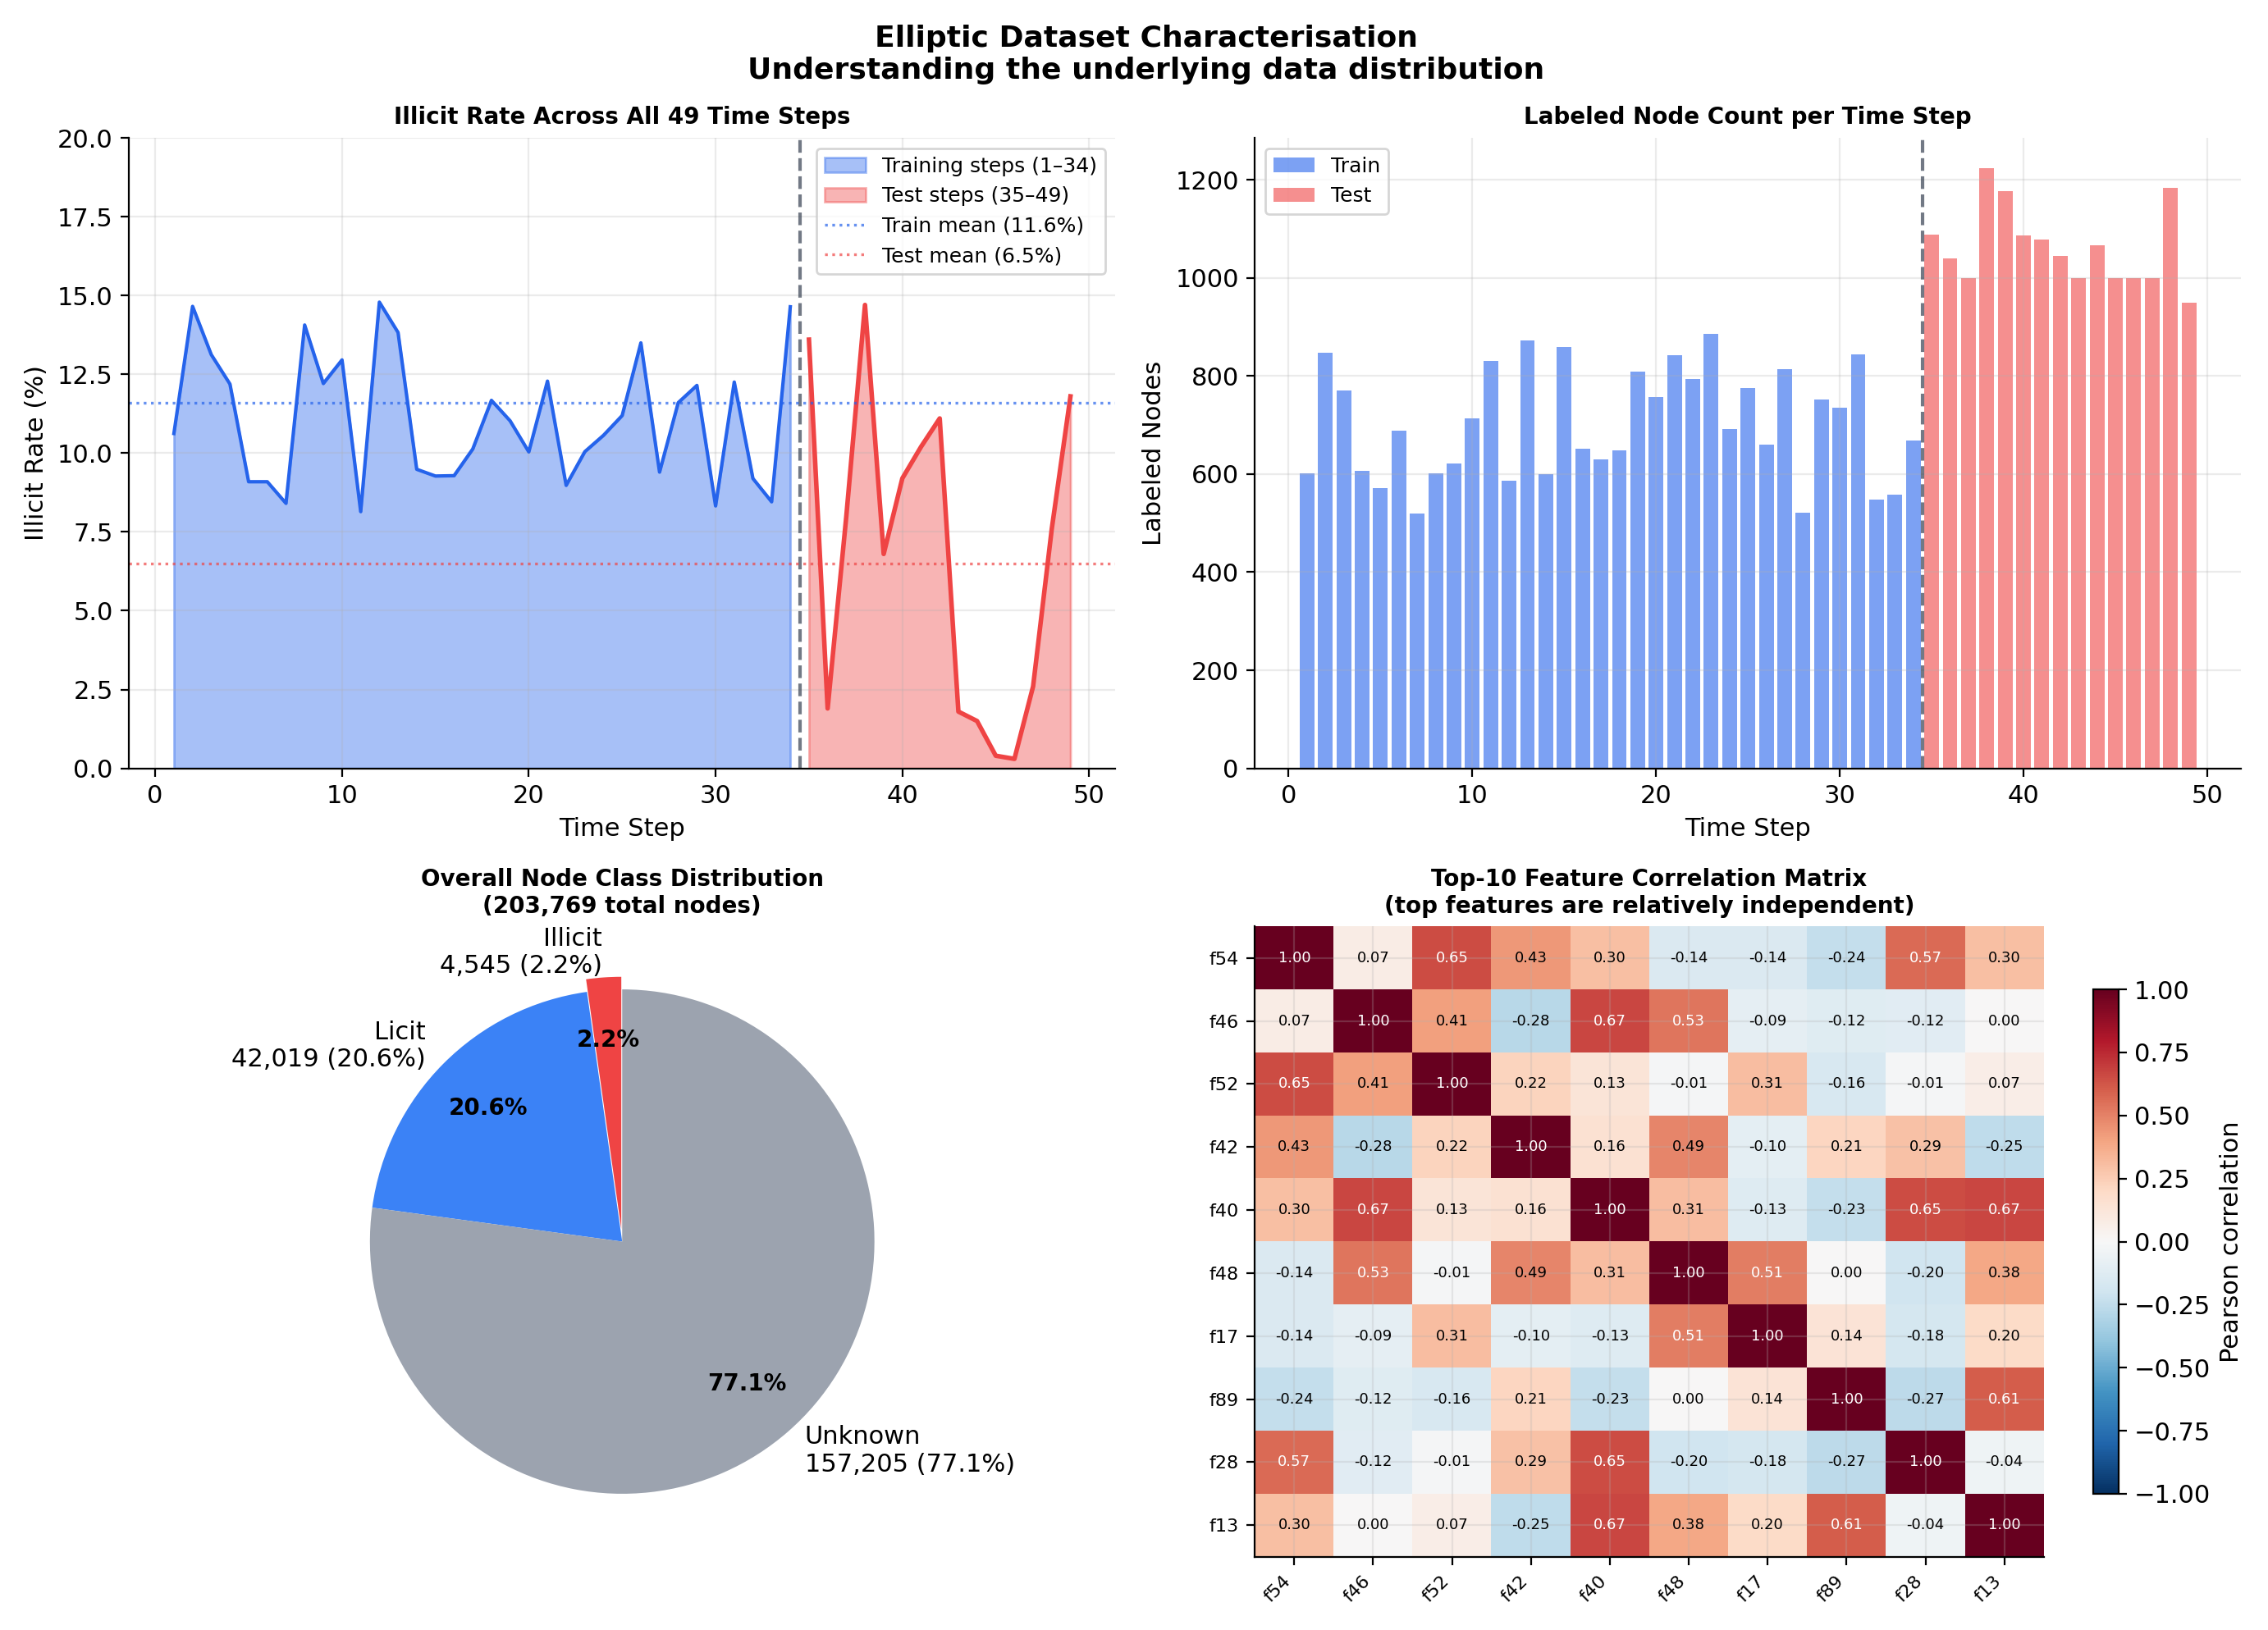
\includegraphics[width=\linewidth]{figures/fig17_dataset_analysis.png}
\caption{Dataset characterisation. The train/test split coincides with
  a fraud-rate regime change. The top features remain informative but
  non-redundant.}
\label{fig:dataset_char}
\end{figure}

%% ---------------------------------------------------------------
\section{Methodology}
\label{sec:methods}

\subsection{Architectures}

\textbf{MLP} (control): 3 hidden layers (128), BatchNorm
\cite{ioffe2015batchnorm}, ReLU, dropout 0.5. Ignores graph
structure; 61,187 parameters. Any MLP--GNN gap isolates the graph
contribution.

\textbf{GCN} \cite{kipf2017}: 2-layer with symmetric degree
normalisation, hidden 128.

\textbf{GraphSAGE} \cite{hamilton2017}: 3-layer mean-aggregation.
Linear(165$\to$256) + [SAGEConv + BN + ReLU + Drop]$\times$3.
Total 438,787 parameters.

\textbf{GAT} \cite{velickovic2018}: 3-layer, 4 attention heads, edge
dropout 0.2, hidden 256, 243,715 parameters. Shows higher seed
variance (std 0.024 vs.\ SAGE's 0.009).

\textbf{EvolveGCN} \cite{pareja2020evolvegcn} (ablation only):
GRU-evolved GCN weights. CPU-constrained to 46,564-node subgraph
with 8 sampled snapshots.

\subsection{Imbalance Strategies}

\textbf{Baseline CE.} Standard cross-entropy, equal weights.

\textbf{Weighted CE.} Square-root inverse-frequency:
$w_c = \sqrt{N_\text{labeled}/2N_c}$, giving
$w_\text{illicit}\approx 2.08$. Linear warmup over 20 epochs.

\textbf{Graph Augmentation.} Clone 30 fraud 1-hop ego-graphs
($\sigma\!=\!0.02$ feature perturbation), attached as isolated
training components.

\subsection{Hybrid Ensembles}

We evaluate four fusion strategies. \emph{GNN alone}: GraphSAGE
weighted. \emph{MLP alone}: no-edges baseline. \emph{Weighted
average}: $\hat{p} = 0.65\,p_\text{GNN} + 0.35\,p_\text{MLP}$.
\emph{Concatenation hybrid}: extract 256-dim GNN embeddings from the
penultimate SAGE layer, concatenate with 165 raw features (421-dim
total), train a Random Forest \cite{breiman2001rf} on the combined
vector.

\subsection{Calibration}

Temperature scaling \cite{guo2017calibration}: optimise scalar $T$
on a held-out set by minimising NLL. Report ECE
\cite{naeini2015calibration} and Brier score before and after.

\subsection{Training}

AdamW \cite{loshchilov2019adamw} ($\text{lr}=10^{-3}$,
wd$=5{\times}10^{-4}$), CosineAnnealingLR, gradient clipping
(max norm 1.0), early stopping patience 30. Inductive evaluation via
RandomNodeLoader (batch 512). All experiments on Apple M4 CPU, 3
seeds. Primary metric: F1 on illicit class
(mean\,$\pm$\,std).

%% ---------------------------------------------------------------
\section{Results}
\label{sec:results}

\subsection{Main Benchmark}

Table~\ref{tab:main_results} and Fig.~\ref{fig:main_results} present
the full 10-configuration benchmark. The MLP (F1\,=\,0.744) beats
GraphSAGE (F1\,=\,0.697) by 4.7 percentage points, well outside both
standard deviations. The MLP has no edges, no neighbourhood
aggregation, no structural signal---yet it leads. The extra structural
processing performed by GNNs hurts rather than helps.

GCN shows an extreme precision paradox: precision 0.89--0.93 but
recall 0.29--0.32. It has learned that predicting licit is almost
always correct, so it does so nearly always. Strategy matters little
for SAGE (all within $\pm$std) but more for GAT, where weighted loss
lifts recall by 5 percentage points.

\begin{figure*}[!t]
\centering
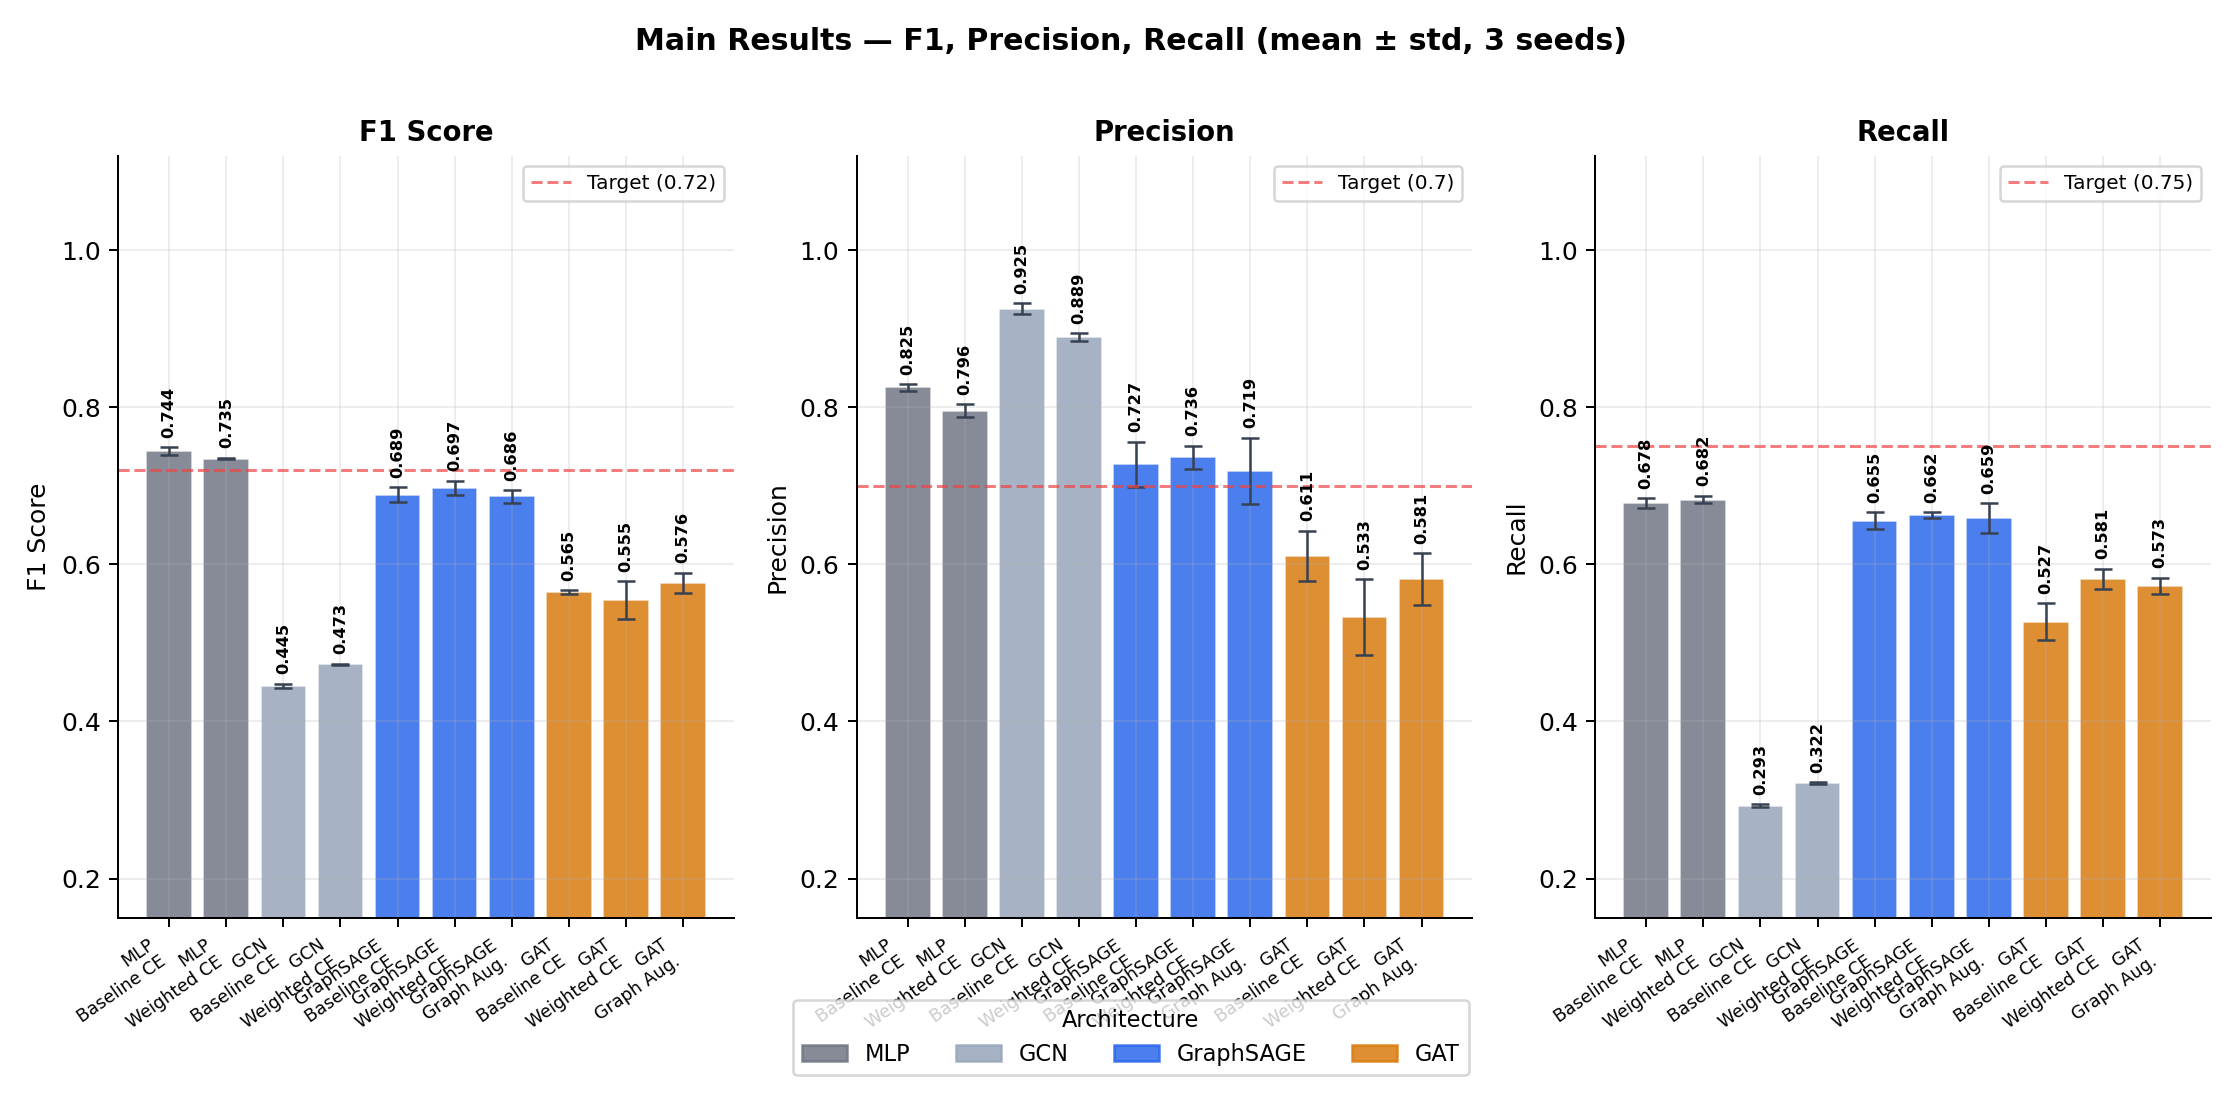
\includegraphics[width=0.96\textwidth]{figures/fig1_main_results.png}
\caption{Main benchmark: F1, Precision, Recall (mean\,$\pm$\,std,
  3 seeds). MLP achieves the highest F1. GCN shows the precision
  paradox: near-perfect precision, near-zero recall. GAT error bars
  are widest, reflecting attention instability under class imbalance.}
\label{fig:main_results}
\end{figure*}

\begin{table*}[!t]
\centering
\caption{Benchmark Results (Mean $\pm$ Std, 3 Seeds). Bold: column
  best. No configuration reaches the 0.75 recall target.}
\label{tab:main_results}
\small
\setlength{\tabcolsep}{5pt}
\begin{tabular}{llrrrr}
\toprule
\textbf{Model} & \textbf{Strategy}
  & \textbf{F1} & \textbf{Prec.}
  & \textbf{Recall} & \textbf{AUC} \\
\midrule
\multirow{2}{*}{MLP}
  & Baseline CE
    & $\mathbf{0.744\pm0.005}$ & $\mathbf{0.825\pm0.004}$
    & $0.678\pm0.006$ & $0.891\pm0.001$ \\
  & Weighted CE
    & $0.735\pm0.001$ & $0.796\pm0.008$
    & $0.682\pm0.005$ & $\mathbf{0.893\pm0.006}$ \\
\midrule
\multirow{2}{*}{GCN}
  & Baseline CE
    & $0.445\pm0.003$ & $0.925\pm0.007$
    & $0.293\pm0.002$ & $0.868\pm0.009$ \\
  & Weighted CE
    & $0.473\pm0.001$ & $0.889\pm0.005$
    & $0.322\pm0.001$ & $0.872\pm0.004$ \\
\midrule
\multirow{3}{*}{GraphSAGE}
  & Baseline CE
    & $0.689\pm0.009$ & $0.727\pm0.029$
    & $0.655\pm0.011$ & $0.867\pm0.006$ \\
  & Weighted CE
    & $0.697\pm0.009$ & $0.736\pm0.015$
    & $0.662\pm0.004$ & $0.868\pm0.003$ \\
  & Graph Aug.
    & $0.686\pm0.008$ & $0.719\pm0.042$
    & $0.659\pm0.019$ & $0.861\pm0.007$ \\
\midrule
\multirow{3}{*}{GAT}
  & Baseline CE
    & $0.565\pm0.002$ & $0.611\pm0.032$
    & $0.527\pm0.023$ & $0.863\pm0.007$ \\
  & Weighted CE
    & $0.555\pm0.024$ & $0.533\pm0.048$
    & $\mathbf{0.581\pm0.013}$ & $0.855\pm0.004$ \\
  & Graph Aug.
    & $0.576\pm0.013$ & $0.581\pm0.033$
    & $0.573\pm0.010$ & $0.842\pm0.002$ \\
\bottomrule
\end{tabular}
\end{table*}

\subsection{Classical and Hybrid Baselines}

Table~\ref{tab:classical} compares against classical models, hybrid
approaches, and prior published results. Random Forest achieves
F1\,=\,0.820 with no graph structure---the strongest single result.
XGBoost reaches F1\,=\,0.775. Our inductive RF exceeds the published
transductive RF (F1\,=\,0.640 \cite{weber2019}) by 18 points, likely
because the original study did not tune RF hyperparameters.

\begin{table}[!t]
\centering
\caption{Classical Baselines, Hybrids, and Prior Work.
  $\dagger$: transductive, GPU. Concat hybrid feeds GNN embeddings
  + raw features into RF.}
\label{tab:classical}
\scriptsize
\setlength{\tabcolsep}{3pt}
\begin{tabular}{llccl}
\toprule
\textbf{Model} & \textbf{Protocol} & \textbf{F1} & \textbf{AUC}
  & \textbf{Graph?} \\
\midrule
LR$^\dagger$ \cite{weber2019}    & Transductive & 0.530 & --- & No \\
RF$^\dagger$ \cite{weber2019}    & Transductive & 0.640 & --- & No \\
\textbf{RF (ours)}        & \textbf{Inductive} & \textbf{0.820}
  & \textbf{0.933} & \textbf{No} \\
XGBoost (ours)            & Inductive & 0.775 & 0.931 & No \\
\midrule
GNN-SAGE (orig.\ graph)   & Inductive & 0.290 & 0.845 & Yes \\
GNN-SAGE (temporal graph)  & Inductive & 0.549 & 0.895 & Yes \\
GNN + RF (emb.\ only)     & Inductive & 0.558 & 0.830 & Yes \\
\textbf{Concat hybrid}    & \textbf{Inductive} & \textbf{0.807}
  & 0.900 & \textbf{Yes} \\
\midrule
GCN$^\dagger$ \cite{weber2019}   & Transductive & 0.700 & --- & Yes \\
EvolveGCN$^\dagger$ \cite{pareja2020evolvegcn} & Temporal & 0.770
  & --- & Yes \\
\bottomrule
\end{tabular}
\end{table}

The concat hybrid (F1\,=\,0.807, precision 0.976) recovers nearly all
performance from components that individually score around 0.31. GNN
embeddings encode different information than raw features; the
downstream RF selectively uses structural signal where it helps and
ignores it where it misleads. Probability-level fusion (weighted
average, F1\,=\,0.453) helps less because it applies the same
weighting everywhere.

\begin{figure}[!t]
\centering
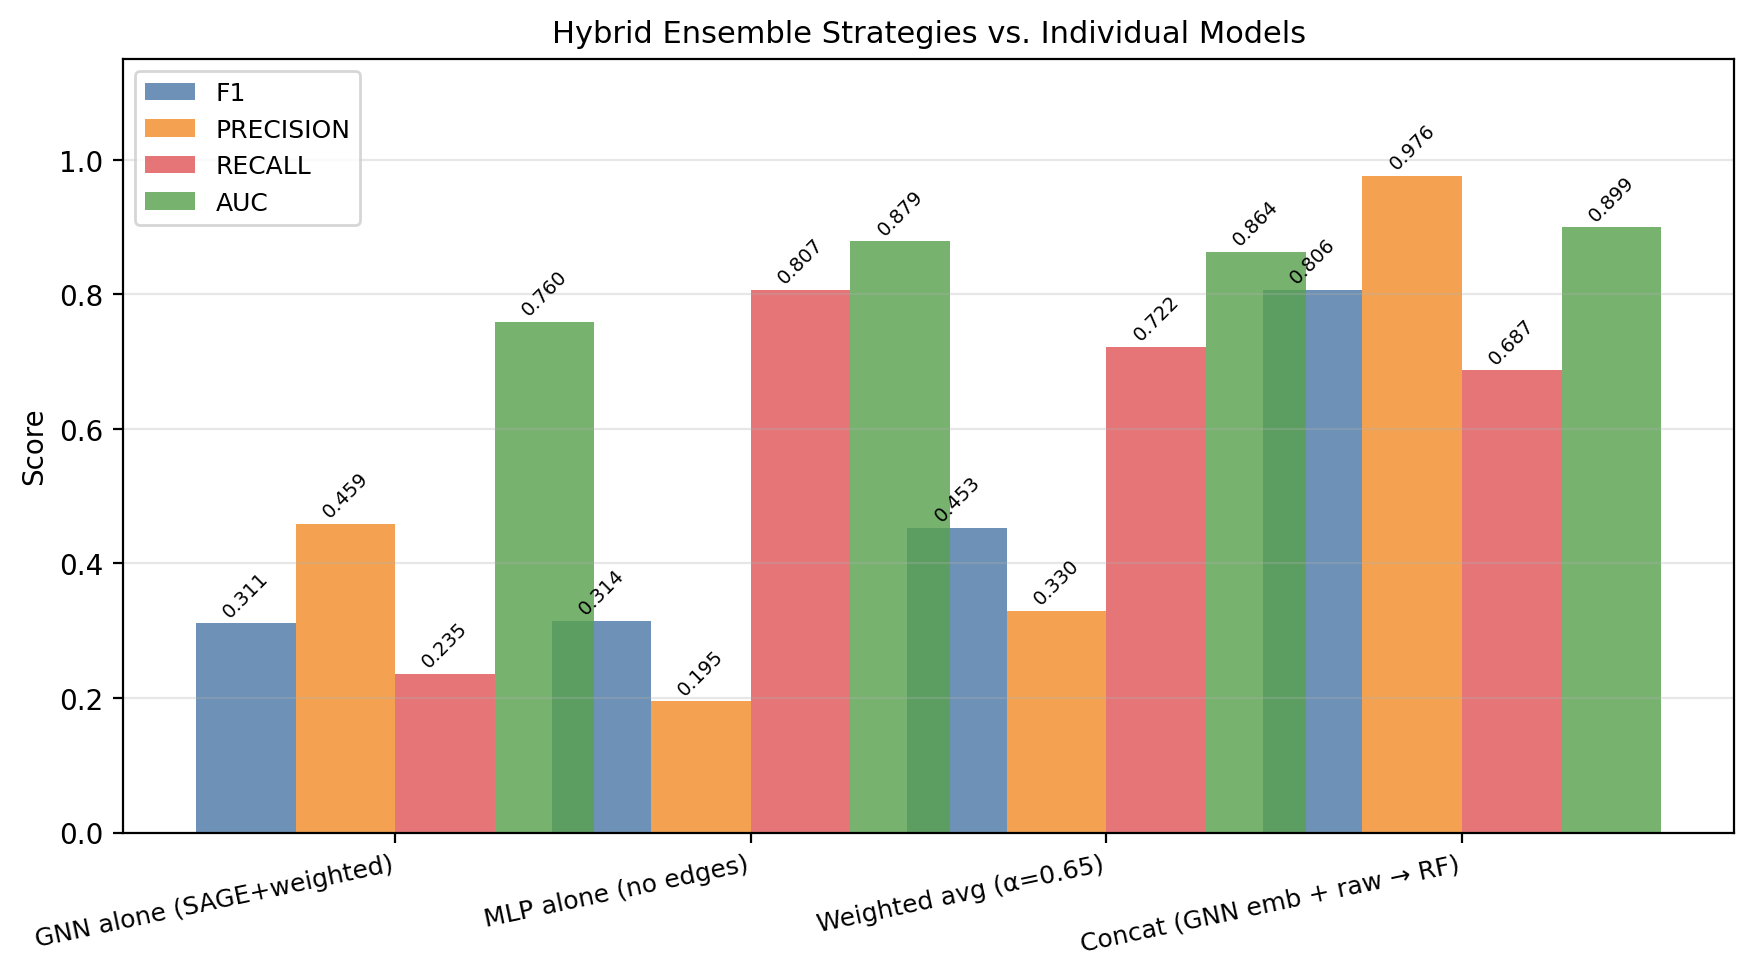
\includegraphics[width=0.92\linewidth]{figures/hybrid_ensemble.png}
\caption{Hybrid ensemble comparison. The concat hybrid (rightmost)
  dramatically outperforms component models. GNN alone and MLP alone
  both score around 0.31; the concat hybrid reaches 0.807.}
\label{fig:hybrid}
\end{figure}

\subsection{Temporal Collapse}

Fig.~\ref{fig:temporal} shows per-step F1 versus true illicit rate.
Every configuration collapses identically after step~42. For
GraphSAGE + Weighted CE: mean F1 falls from 0.799 (steps 35--42) to
0.012 (steps 43--49). The collapse is a recall failure: predicted
fraud rate drops from 8.2\,\% to 1.7\,\%. Models stop predicting
fraud rather than becoming confused.

\begin{figure*}[!t]
\centering
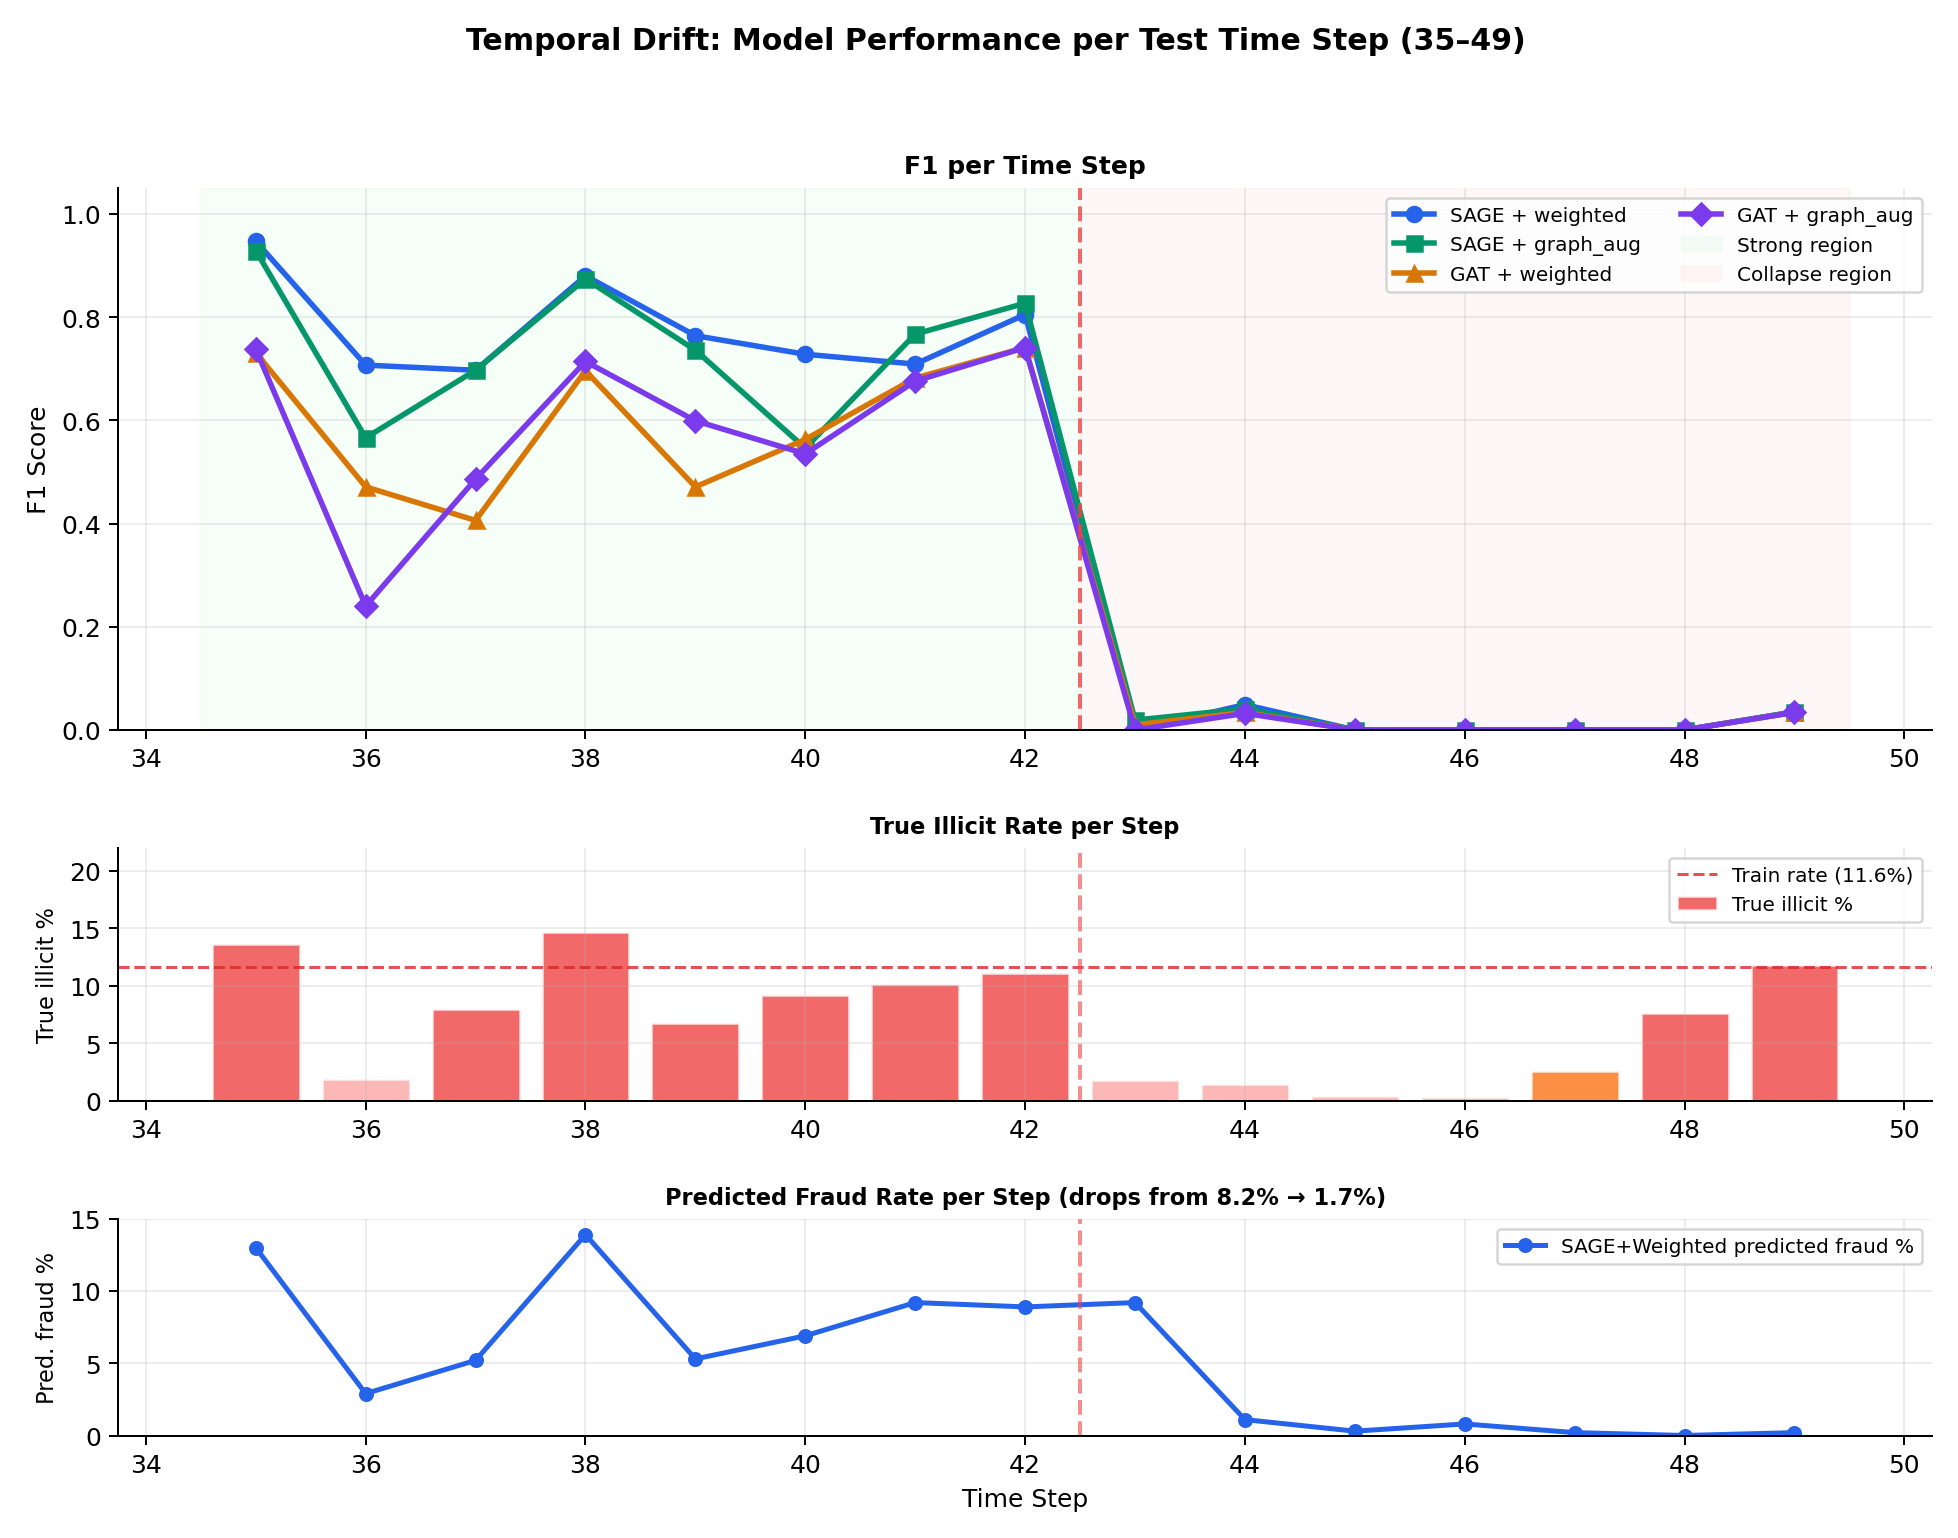
\includegraphics[width=0.96\textwidth]{figures/fig2_temporal_drift.png}
\caption{Per-step F1 (top) versus true illicit rate (bottom). All
  configurations collapse identically after step~42, directly
  corresponding to the fraud-rate drop below 2\,\%. Architecture and
  strategy differences vanish at the collapse boundary.}
\label{fig:temporal}
\end{figure*}

For GraphSAGE + Weighted CE, the per-step numbers are stark: steps
35--42 average F1\,=\,0.799 (with step~35 reaching 0.947), while
steps 43--49 average F1\,=\,0.012. Step~46 has only 3 fraud nodes
among 960 labeled transactions (0.3\,\%); the model stops predicting
fraud at that base rate, rendering it operationally useless. The
predicted fraud rate drops from 8.2\,\% to 1.7\,\%---not confusion
but systematic underconfidence.

%% ---------------------------------------------------------------
\section{Analysis}
\label{sec:analysis}

\subsection{Feature Attribution}

Random Forest importance on all 165 features
(Fig.~\ref{fig:analysis_pair}a) reveals that local features
($f_0$--$f_{93}$) account for 82.4\,\% of total Gini importance.
Aggregate neighbourhood features contribute only 17.6\,\% despite
directly encoding 1-hop summaries. The top 17 features explain
50\,\% of cumulative importance; the most important feature (f54,
importance 0.056) is local. The implication is direct: the signal
that matters for classification is concentrated in features accessible
to the MLP, while the GNN's structural component introduces
topological patterns from the training period that become misleading
under shift.

\subsection{Graph-Structure Ablation}

Table~\ref{tab:ablation} presents the most surprising result.
GraphSAGE trained with randomly shuffled edges (same count, random
endpoints) achieves F1\,=\,0.383, outperforming both original edges
(0.268, $\Delta = +0.116$) and no edges (0.332). The original
transaction graph is the worst of the three conditions.

\begin{table}[!t]
\centering
\caption{Multi-Seed Graph-Structure Ablation (3 Seeds Each). Shuffled
  edges outperform original edges by 11.6 F1 points. Random wiring is
  better than real wiring.}
\label{tab:ablation}
\small
\begin{tabular}{lrrrr}
\toprule
\textbf{Condition} & \textbf{F1} & \textbf{Prec.}
  & \textbf{Recall} & \textbf{AUC} \\
\midrule
Original graph
  & $0.268 \pm 0.030$ & $0.163 \pm 0.020$
  & $0.745 \pm 0.074$ & $0.825 \pm 0.047$ \\
Shuffled edges
  & $\mathbf{0.383 \pm 0.023}$ & $\mathbf{0.258 \pm 0.022}$
  & $\mathbf{0.754 \pm 0.007}$ & $\mathbf{0.884 \pm 0.003}$ \\
No edges (MLP)
  & $0.332 \pm 0.018$ & $0.210 \pm 0.015$
  & $0.799 \pm 0.007$ & $0.878 \pm 0.003$ \\
\bottomrule
\end{tabular}
\end{table}

The original graph's mean degree of 2.3 produces neighbourhoods that
are sparse and semantically misleading under shift. Shuffled edges
break this misleading structure while providing regularisation through
neighbourhood averaging---essentially stochastic feature-space
dropout.

\begin{figure*}[!t]
\centering
\begin{minipage}[b]{0.48\textwidth}
  \centering
  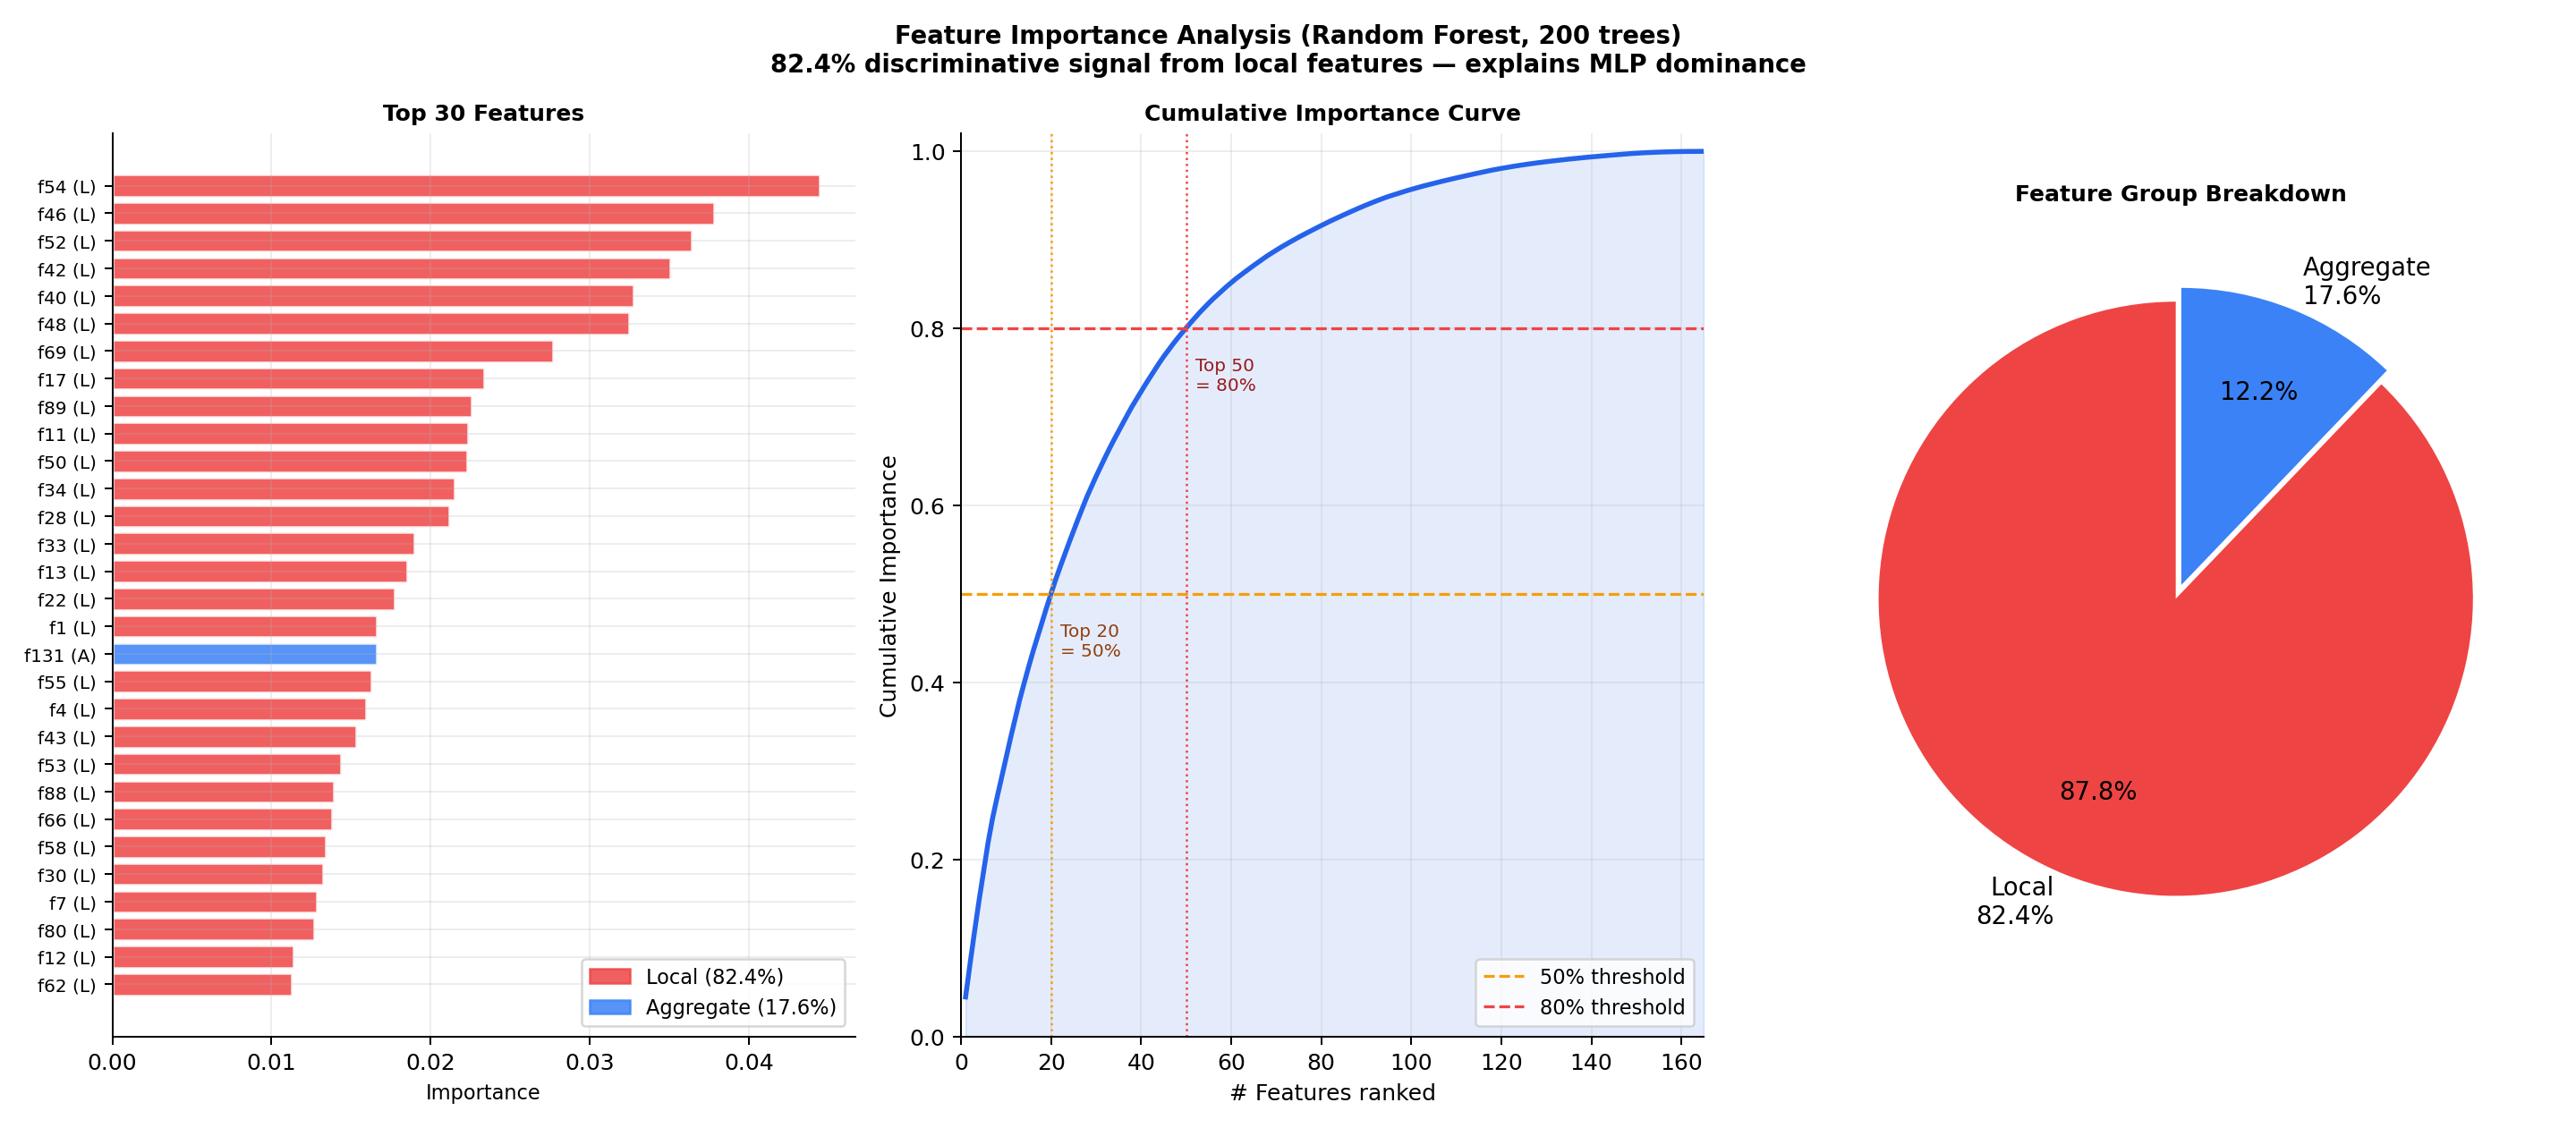
\includegraphics[width=\linewidth]{figures/fig4_feature_importance.png}\\[-0.2em]
  \footnotesize\textbf{(a)} Feature importance. Local features dominate.
\end{minipage}
\hfill
\begin{minipage}[b]{0.48\textwidth}
  \centering
  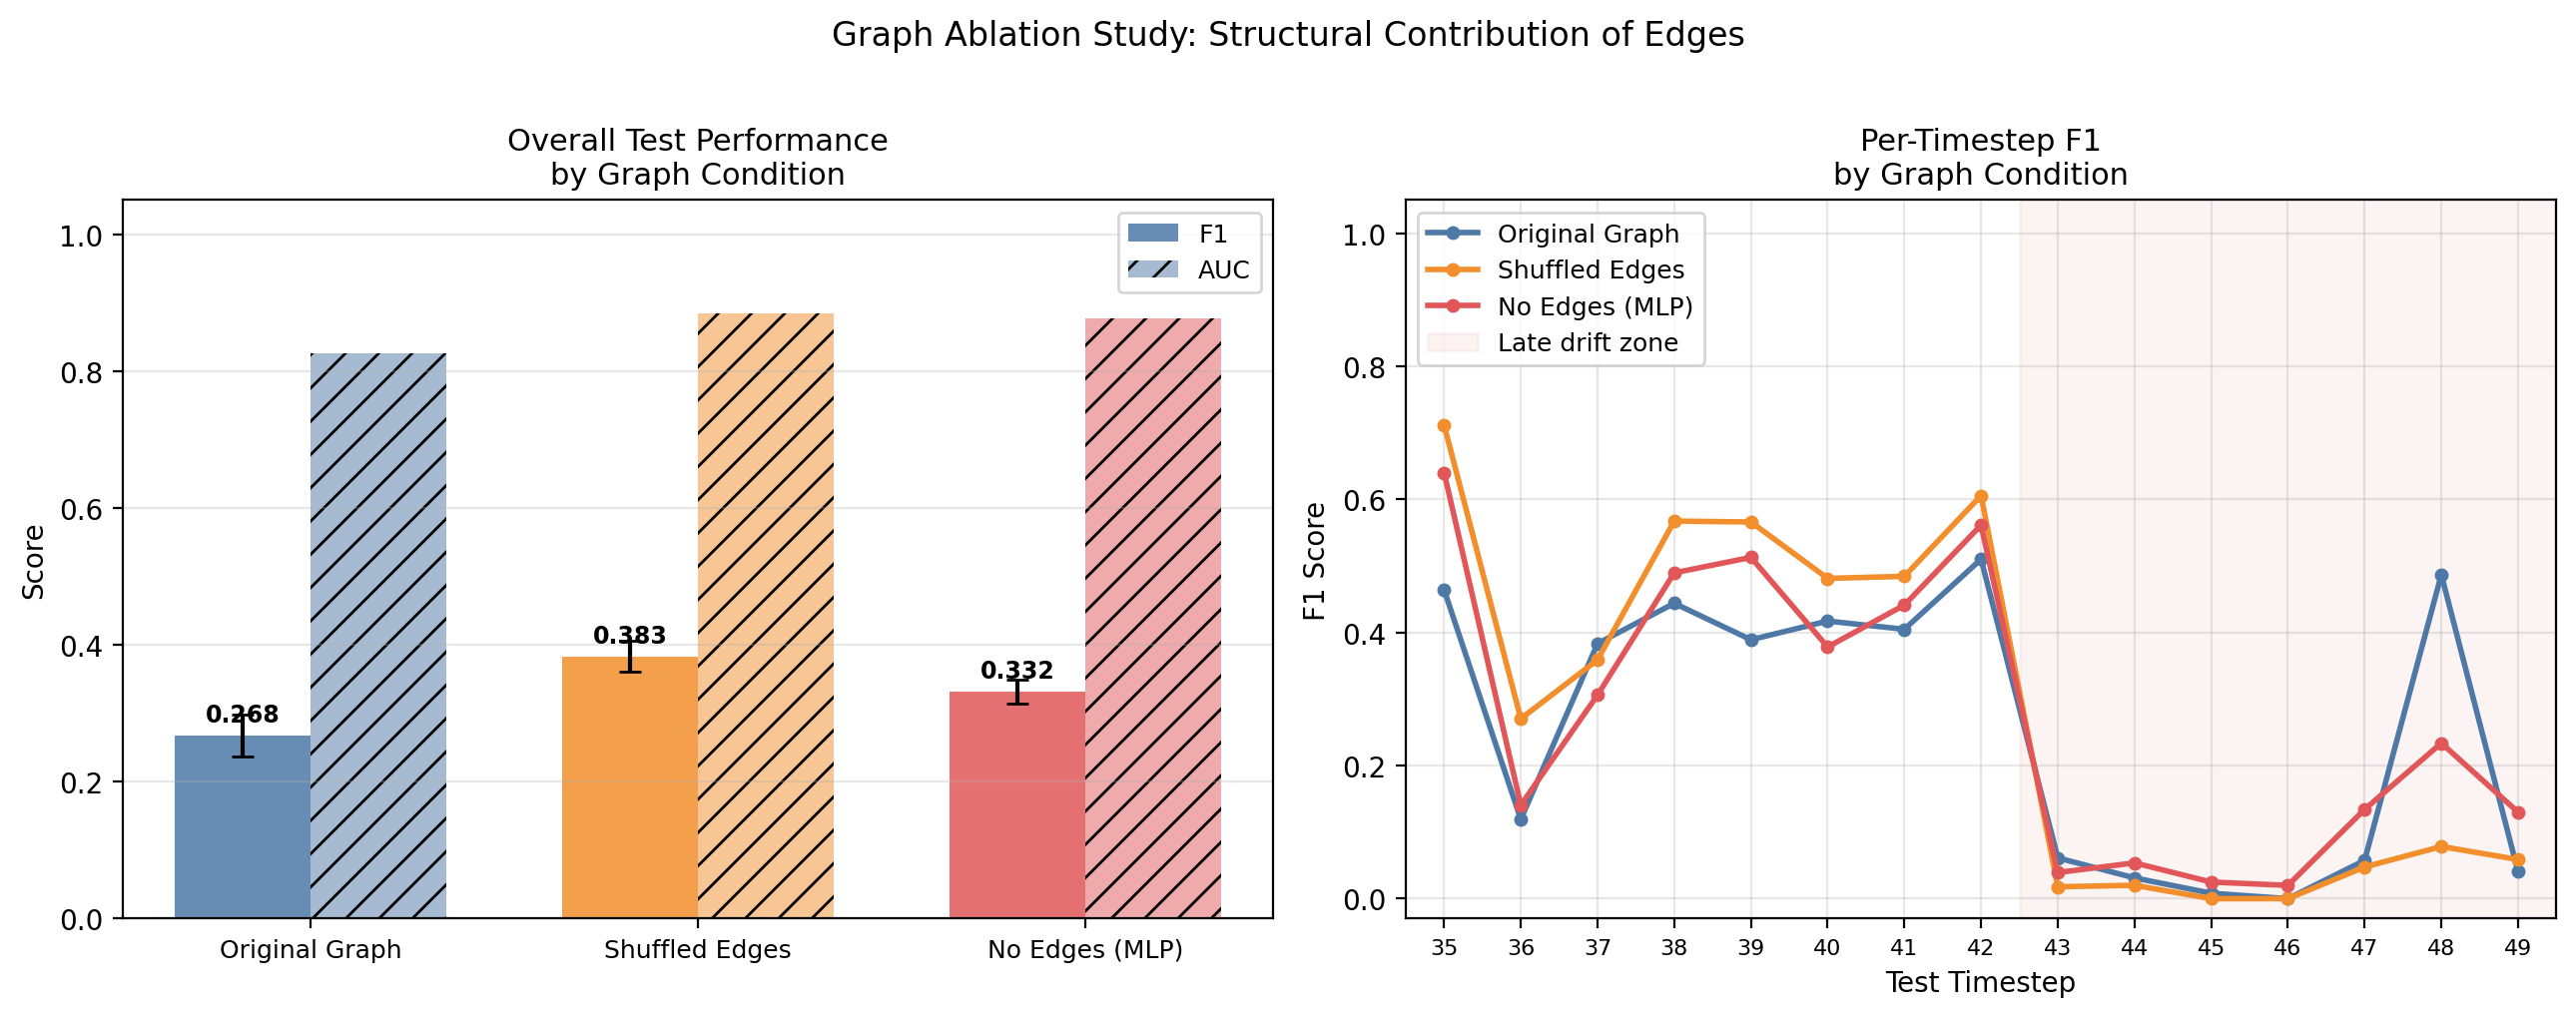
\includegraphics[width=\linewidth]{figures/graph_ablation_extended.png}\\[-0.2em]
  \footnotesize\textbf{(b)} Graph ablation temporal profile (3 seeds).
\end{minipage}
\caption{Left: RF importance shows 82.4\,\% of discriminative power
  sits in local features. Right: shuffled edges outperform original
  edges across most steps; all conditions collapse after step~42.}
\label{fig:analysis_pair}
\end{figure*}

\subsection{Community Structure}

Fraud community structure is real: fraud nodes have 54\,\% fraudulent
neighbours versus 0.56\,\% for licit nodes---a 96$\times$ ratio
(Fig.~\ref{fig:supporting}a). GNNs exploit this during steps 35--42.
The structure becomes a liability in steps 43--49 when learned
topological patterns from training no longer match the test-period
fraud distribution.

\subsection{Calibration}

Temperature scaling yields $\Delta$F1\,=\,0 for all configurations
(Fig.~\ref{fig:supporting}b). Optimal temperatures cluster near 1.0
($T \in [1.03, 1.04]$), indicating only mild overconfidence. ECE
changes by less than 0.002 after scaling. The collapse cannot be
fixed by probability rescaling because temperature scaling is
rank-preserving: it cannot move predictions across the 0.5 threshold
when the model has already stopped assigning fraud probabilities above
that boundary.

\begin{table}[!t]
\centering
\caption{Temperature Scaling Results. ECE reduction is negligible.
  Calibration cannot address the temporal collapse.}
\label{tab:calibration}
\footnotesize
\begin{tabular}{lrrrrr}
\toprule
\textbf{Model} & $T^*$ & \textbf{ECE$_\text{b}$}
  & \textbf{ECE$_\text{a}$} & \textbf{Brier$_\text{b}$}
  & \textbf{Brier$_\text{a}$} \\
\midrule
SAGE wt.   & 1.041 & 0.284 & 0.282 & 0.161 & 0.158 \\
SAGE aug.  & 0.919 & 0.173 & 0.175 & 0.146 & 0.149 \\
GAT wt.    & 1.037 & 0.246 & 0.245 & 0.155 & 0.153 \\
GAT aug.   & 1.027 & 0.266 & 0.266 & 0.157 & 0.156 \\
\bottomrule
\end{tabular}
\end{table}

\subsection{EvolveGCN Hardware Ablation}

CPU-constrained EvolveGCN achieves F1\,=\,0.29, falling 0.48 points
below the published GPU result (F1\,=\,0.77
\cite{pareja2020evolvegcn}). The gap reflects operating on the
46,564-node subgraph with only 8 sampled snapshots rather than the
full graph with all 34.

\begin{figure*}[!t]
\centering
\begin{minipage}[b]{0.32\textwidth}
  \centering
  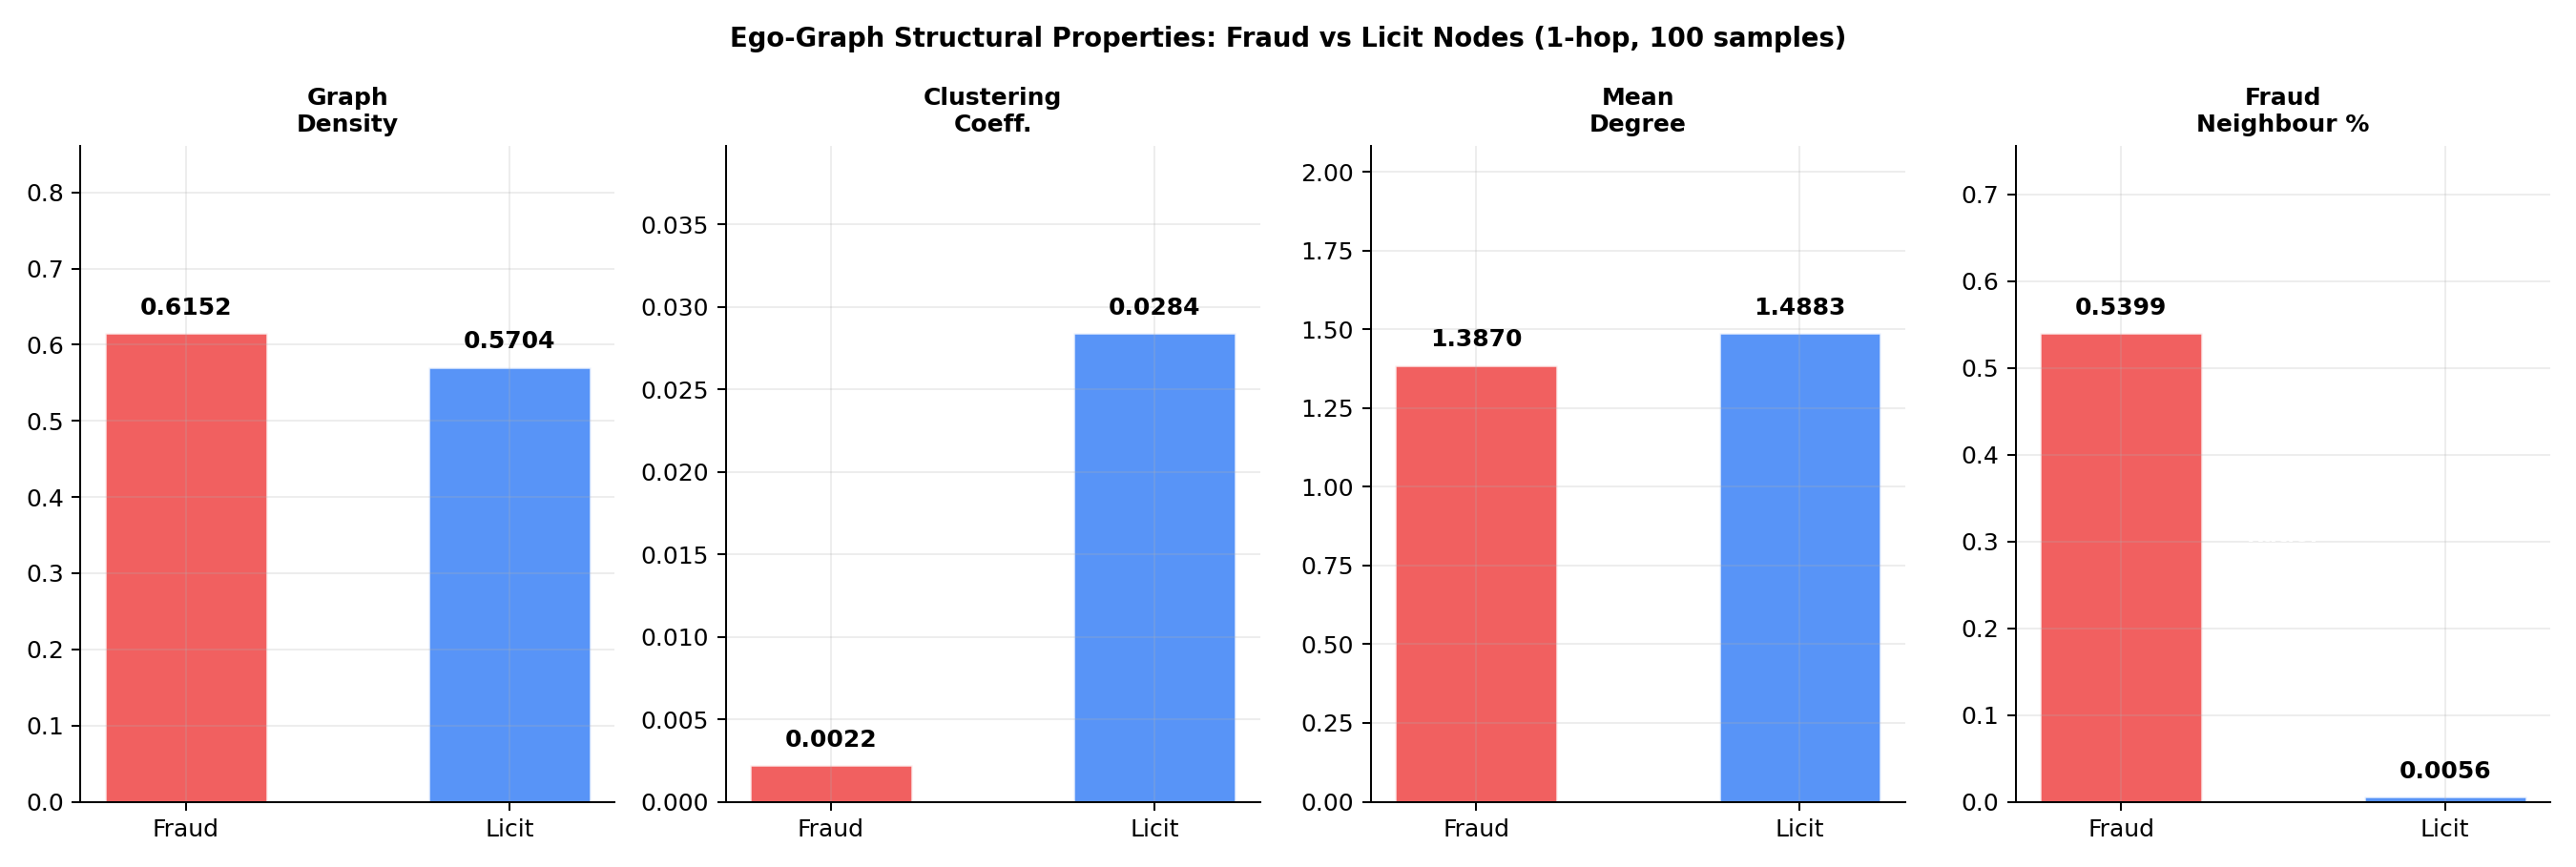
\includegraphics[width=\linewidth]{figures/fig5_community_structure.png}\\[-0.2em]
  \footnotesize\textbf{(a)} Community structure.
\end{minipage}
\hfill
\begin{minipage}[b]{0.32\textwidth}
  \centering
  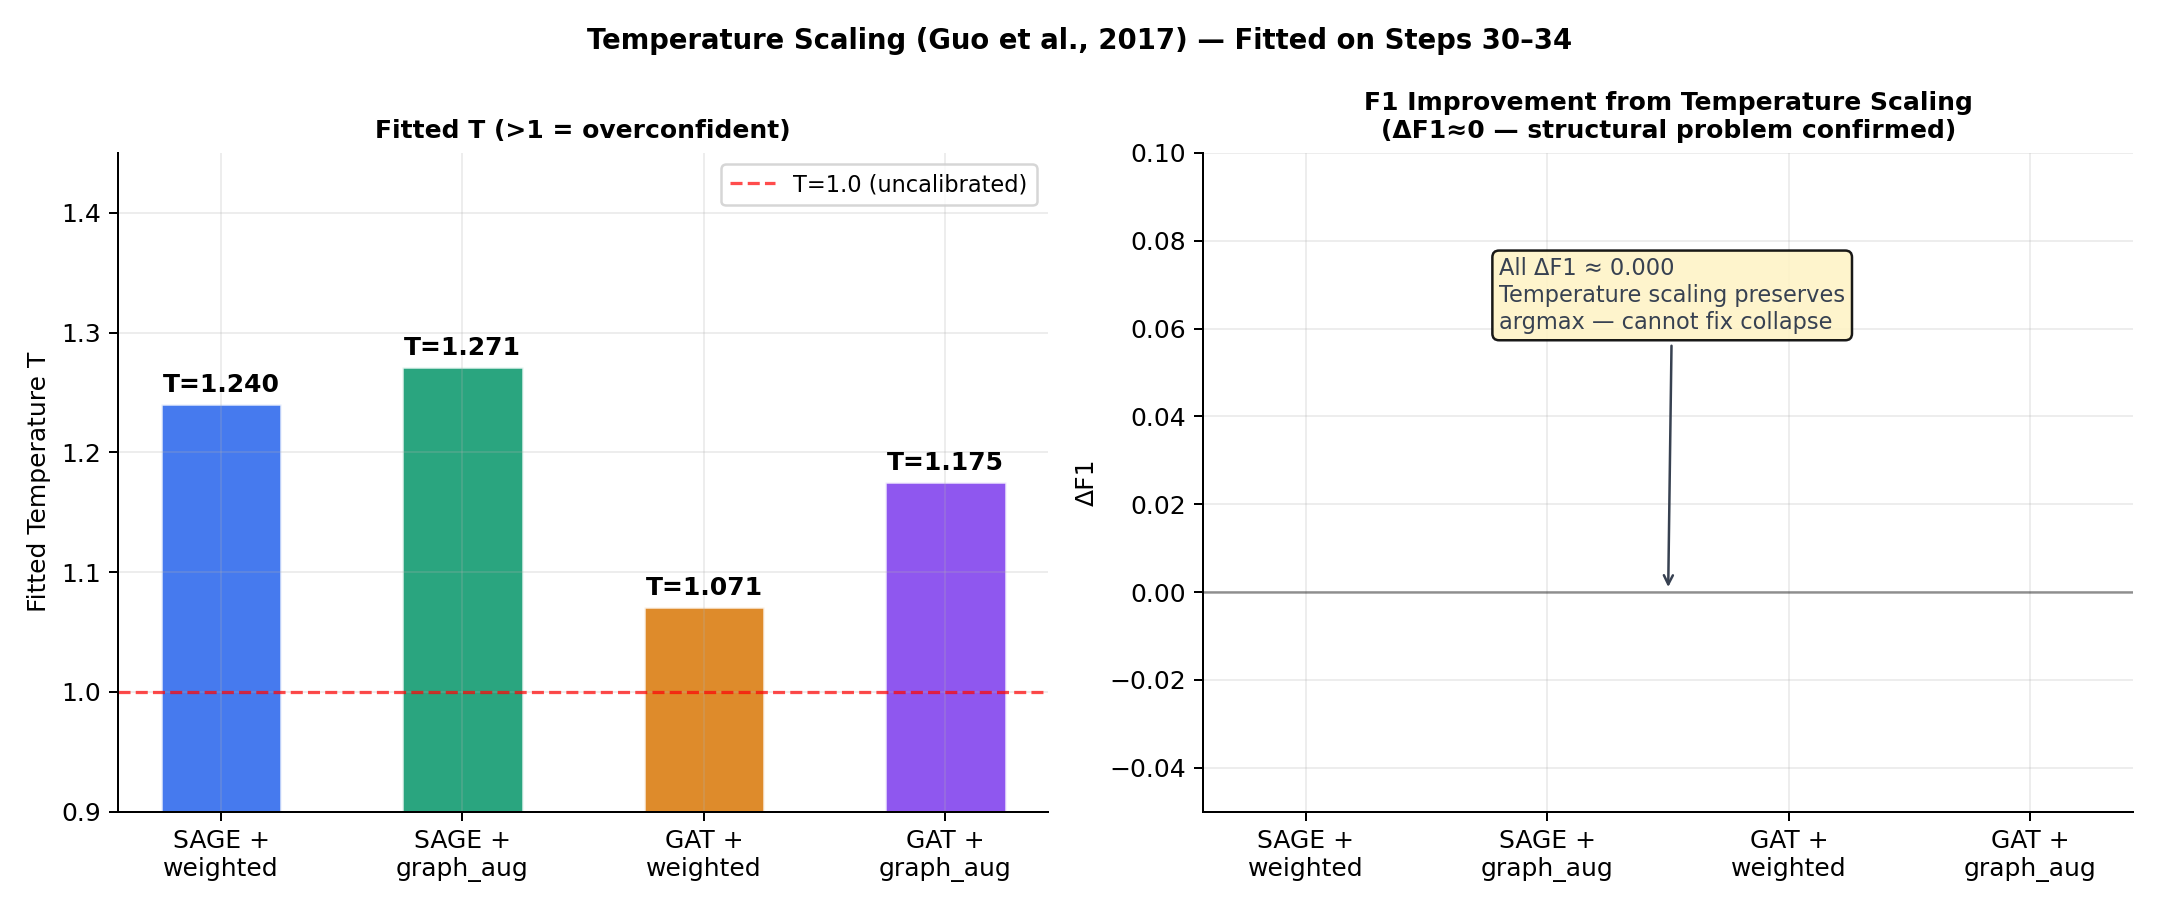
\includegraphics[width=\linewidth]{figures/fig13_temperature_scaling.png}\\[-0.2em]
  \footnotesize\textbf{(b)} Temperature scaling.
\end{minipage}
\hfill
\begin{minipage}[b]{0.32\textwidth}
  \centering
  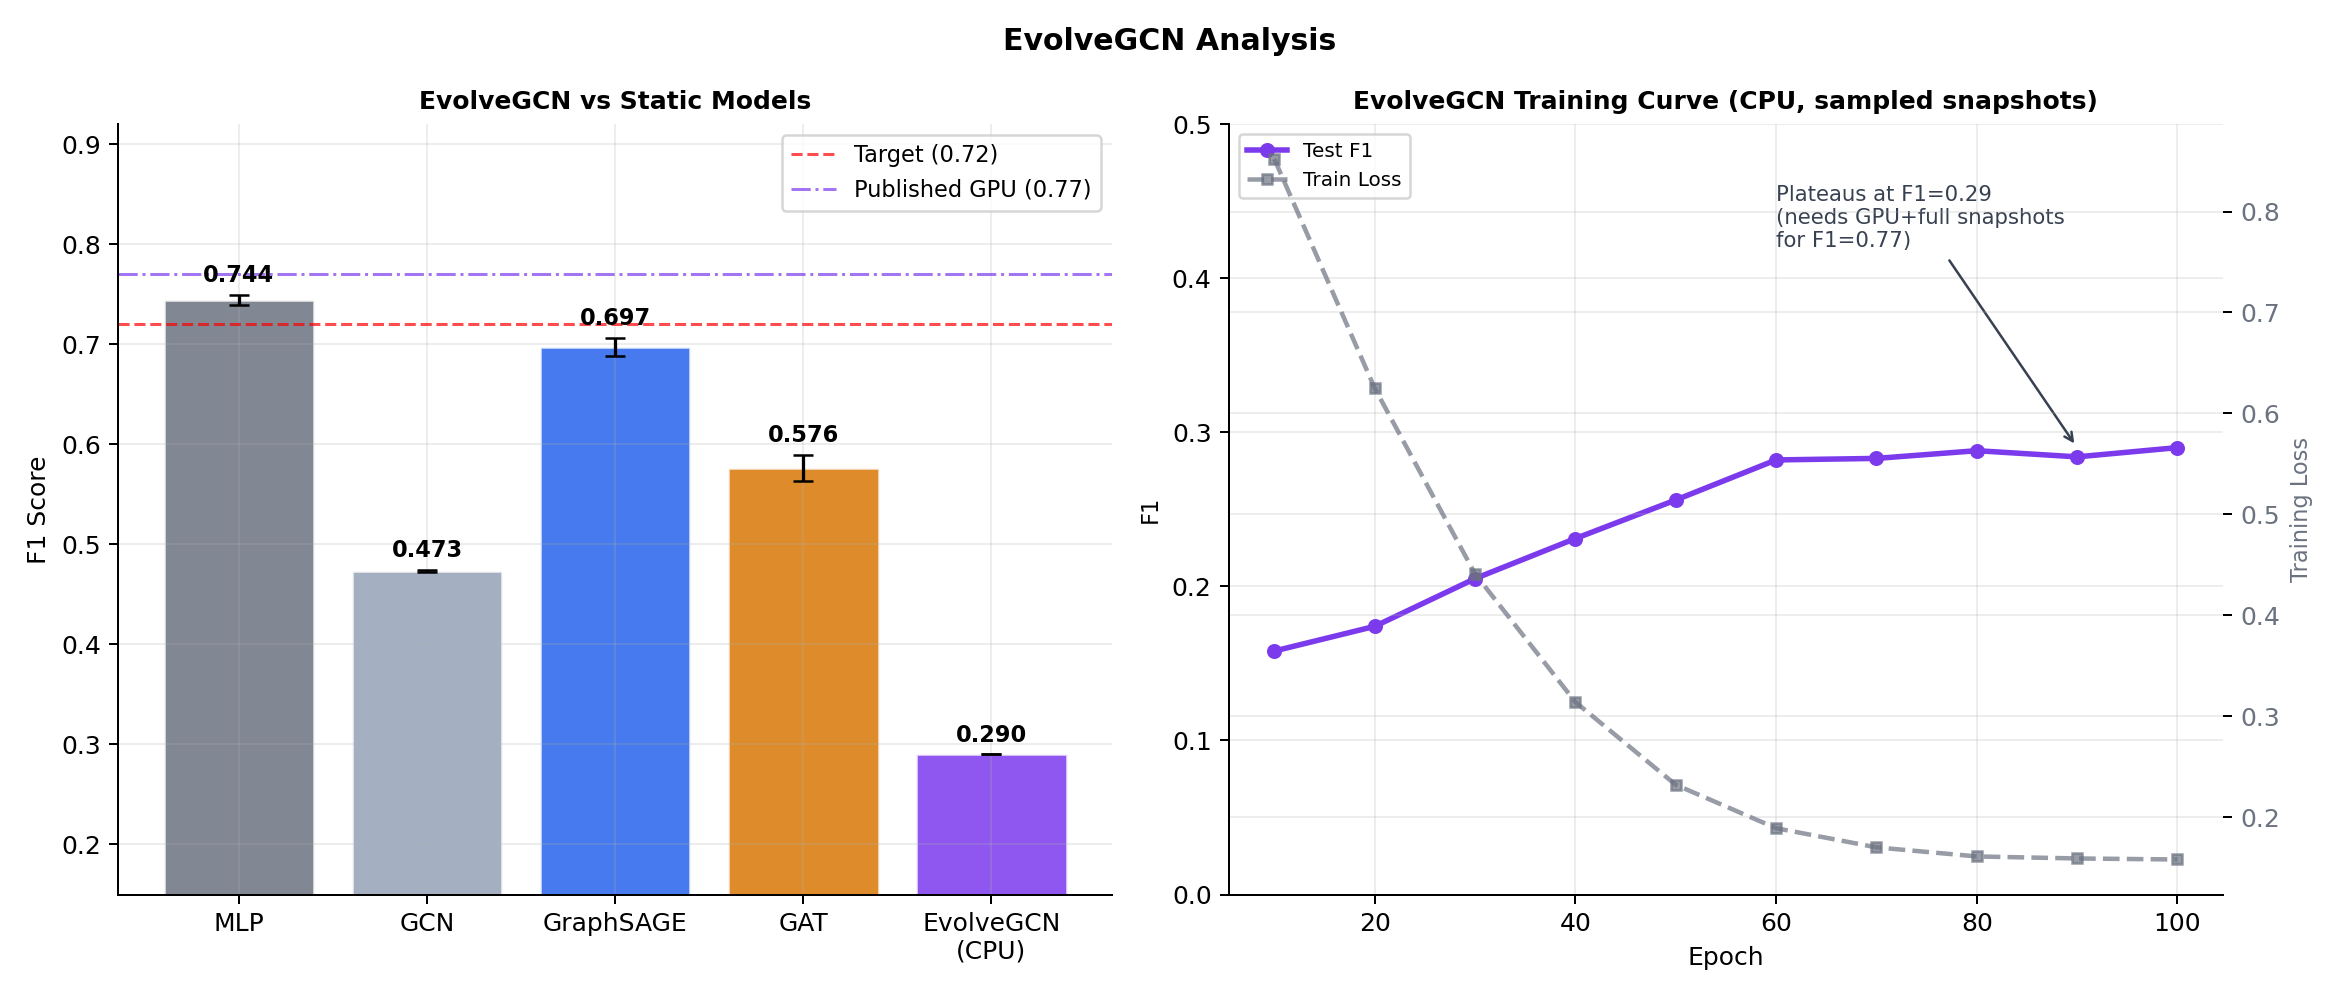
\includegraphics[width=\linewidth]{figures/fig9_evolvegcn.png}\\[-0.2em]
  \footnotesize\textbf{(c)} EvolveGCN hardware ablation.
\end{minipage}
\caption{Supporting analyses. (a) Fraud communities are real but
  temporally fragile. (b) Temperature scaling does not recover
  performance ($\Delta$F1\,=\,0). (c) Temporal GNNs require full
  hardware and snapshot availability.}
\label{fig:supporting}
\end{figure*}

\subsection{Business Cost Analysis}

Under FN\,=\,\$50k and FP\,=\,\$2k, GAT + Graph Aug.\ achieves the
lowest total cost (\$18.5M) despite lower aggregate F1 than SAGE
(Fig.~\ref{fig:biz}). It catches 83 more fraud cases (583 vs.\ 500
TP) with only 103 additional false alarms (558 vs.\ 455 FP). At a
25:1 cost asymmetry, each extra true positive outweighs 25 additional
false alarms.

\begin{figure}[!t]
\centering
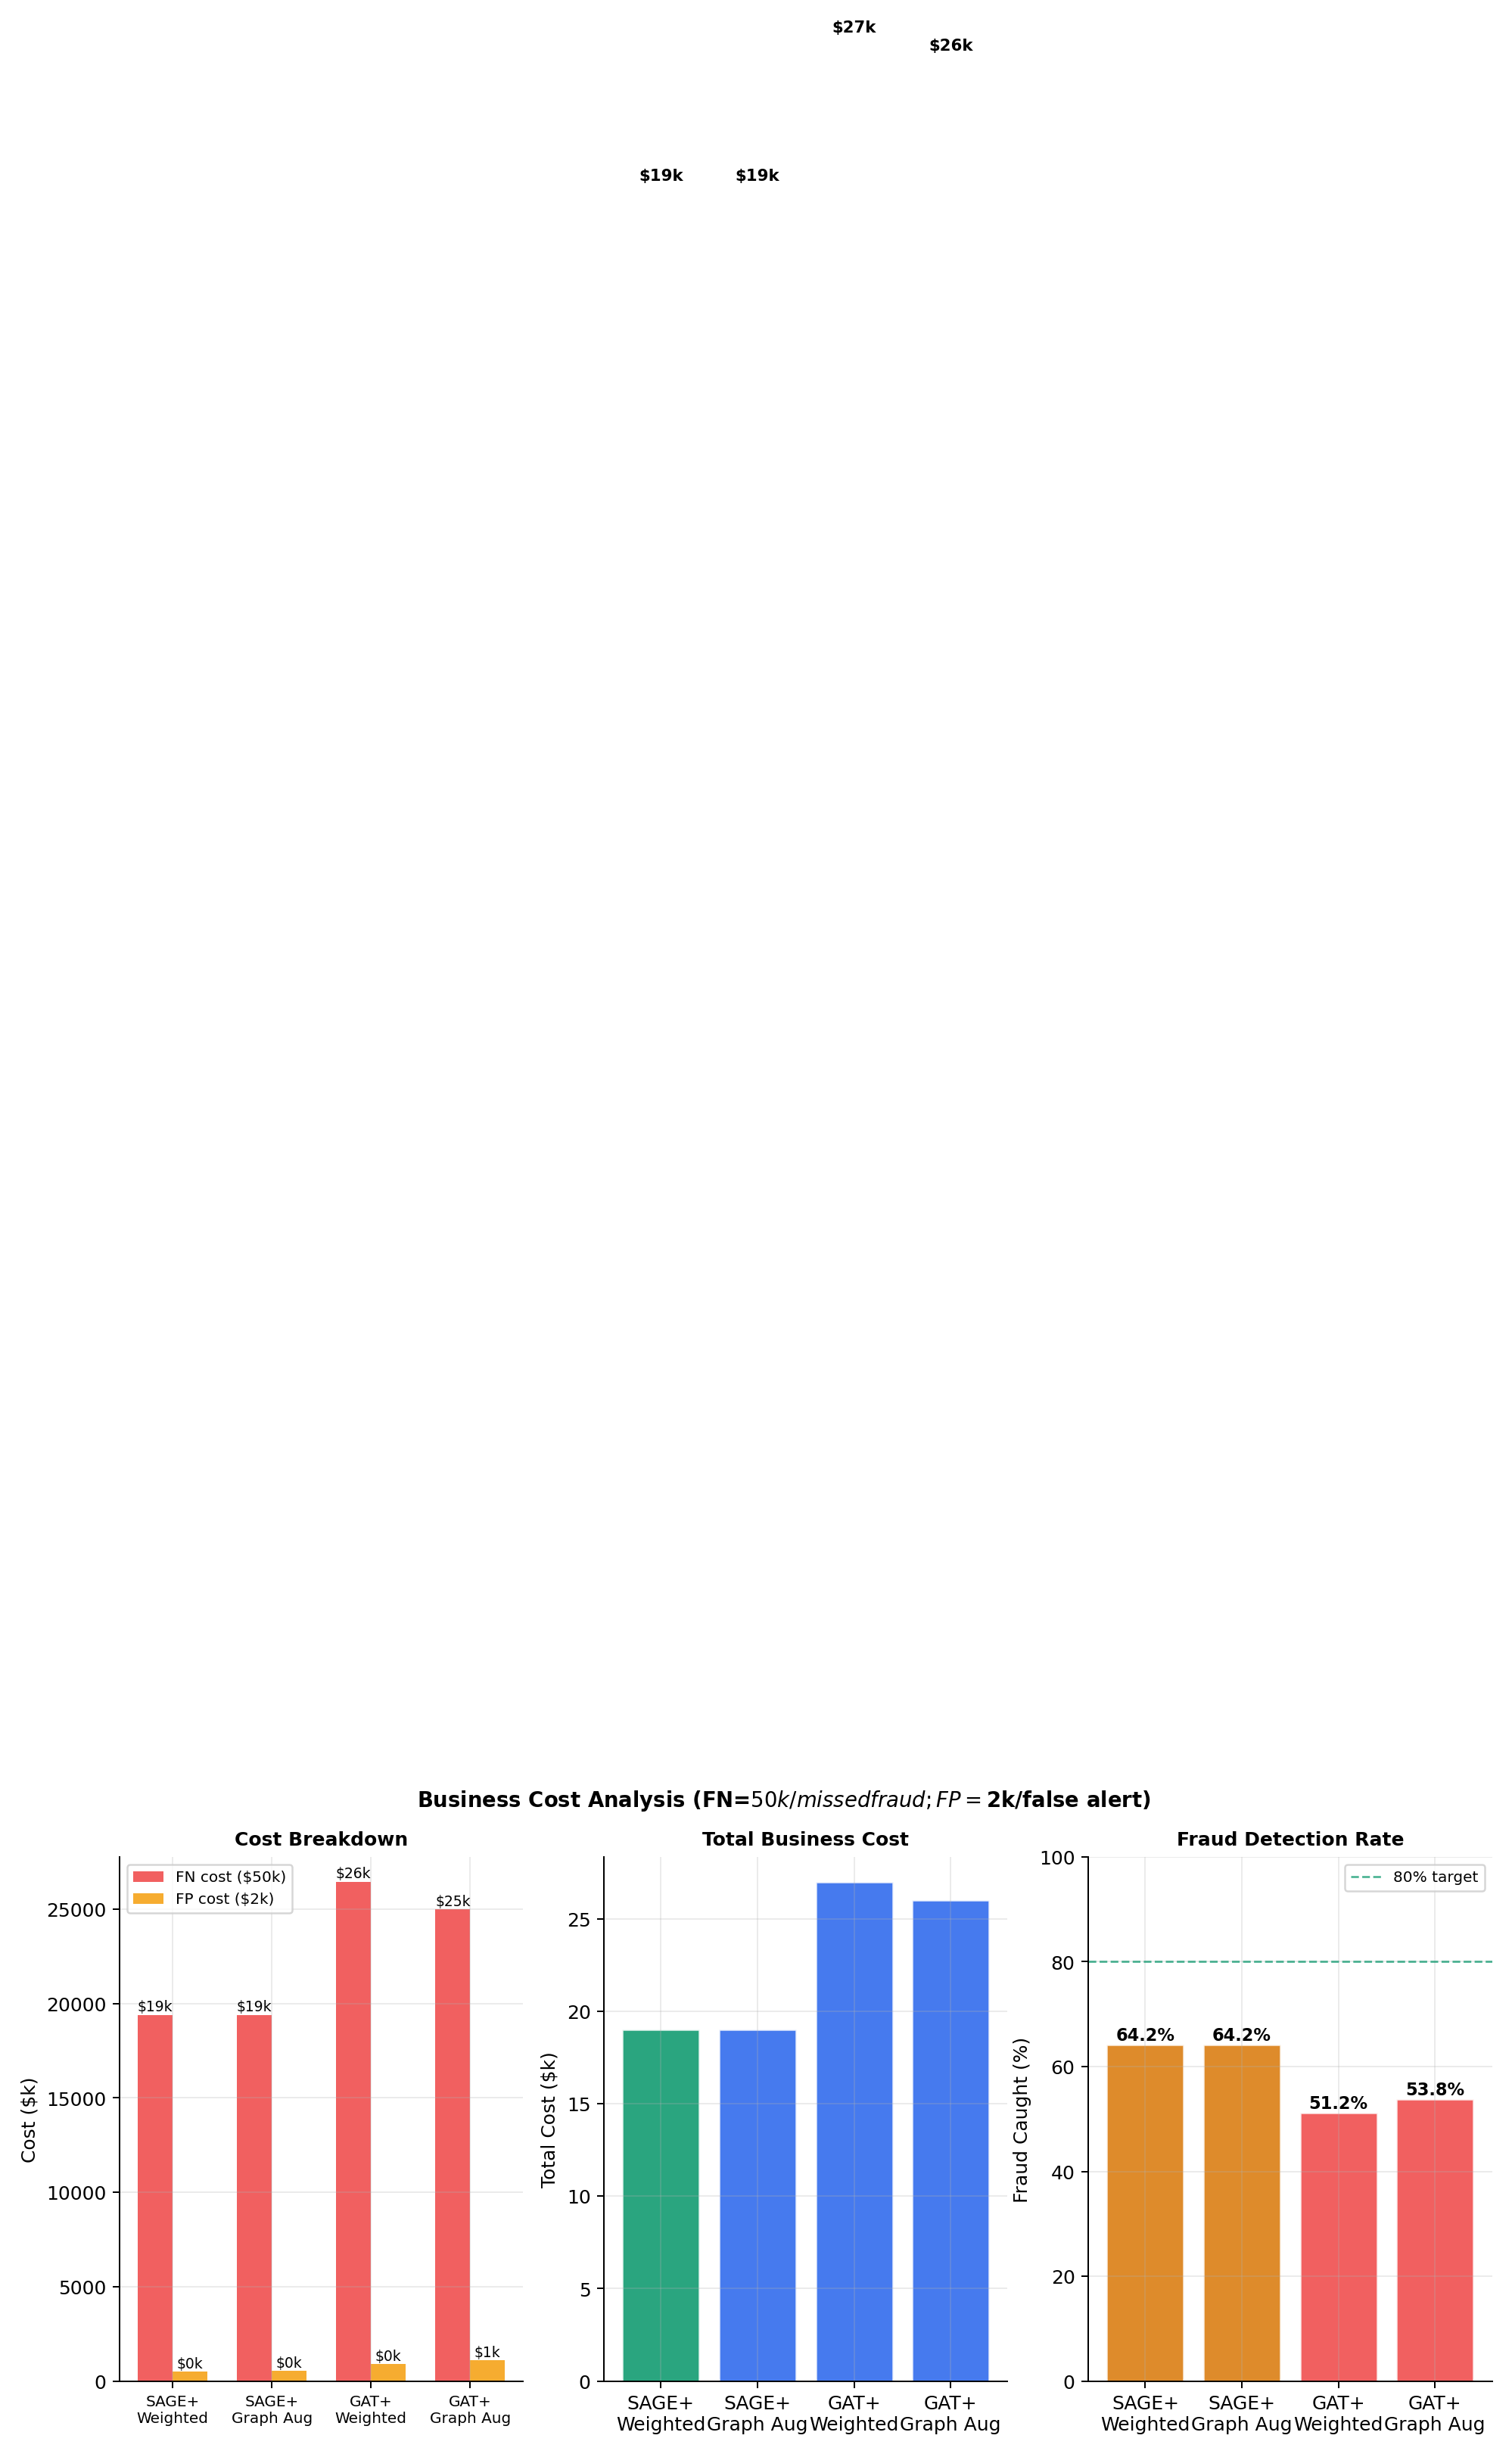
\includegraphics[width=0.90\linewidth]{figures/fig7_business_cost.png}
\caption{Business cost analysis (FN\,=\,\$50k, FP\,=\,\$2k). GAT +
  Graph Aug.\ achieves the lowest operational cost despite lower F1,
  because catching more fraud outweighs the extra false-alarm cost.}
\label{fig:biz}
\end{figure}

\subsection{PR Curves, Confusion Matrices, and Seed Robustness}

SAGE + Graph Aug.\ achieves the highest average precision
(AP\,=\,0.607), indicating better probability ranking despite similar
aggregate F1. No single threshold achieves precision $>$0.70 and
recall $>$0.75 simultaneously (Fig.~\ref{fig:pr_cm}a). Confusion
matrices confirm SAGE produces fewer false negatives (FN\,=\,388)
than GAT (FN\,=\,500--529). Across seeds, MLP and SAGE remain
stable; GAT shows wider variance (Fig.~\ref{fig:pr_cm}b), making
operational tuning harder. Weighted CE is the most consistently
useful imbalance strategy.

\begin{figure*}[!t]
\centering
\begin{minipage}[b]{0.48\textwidth}
  \centering
  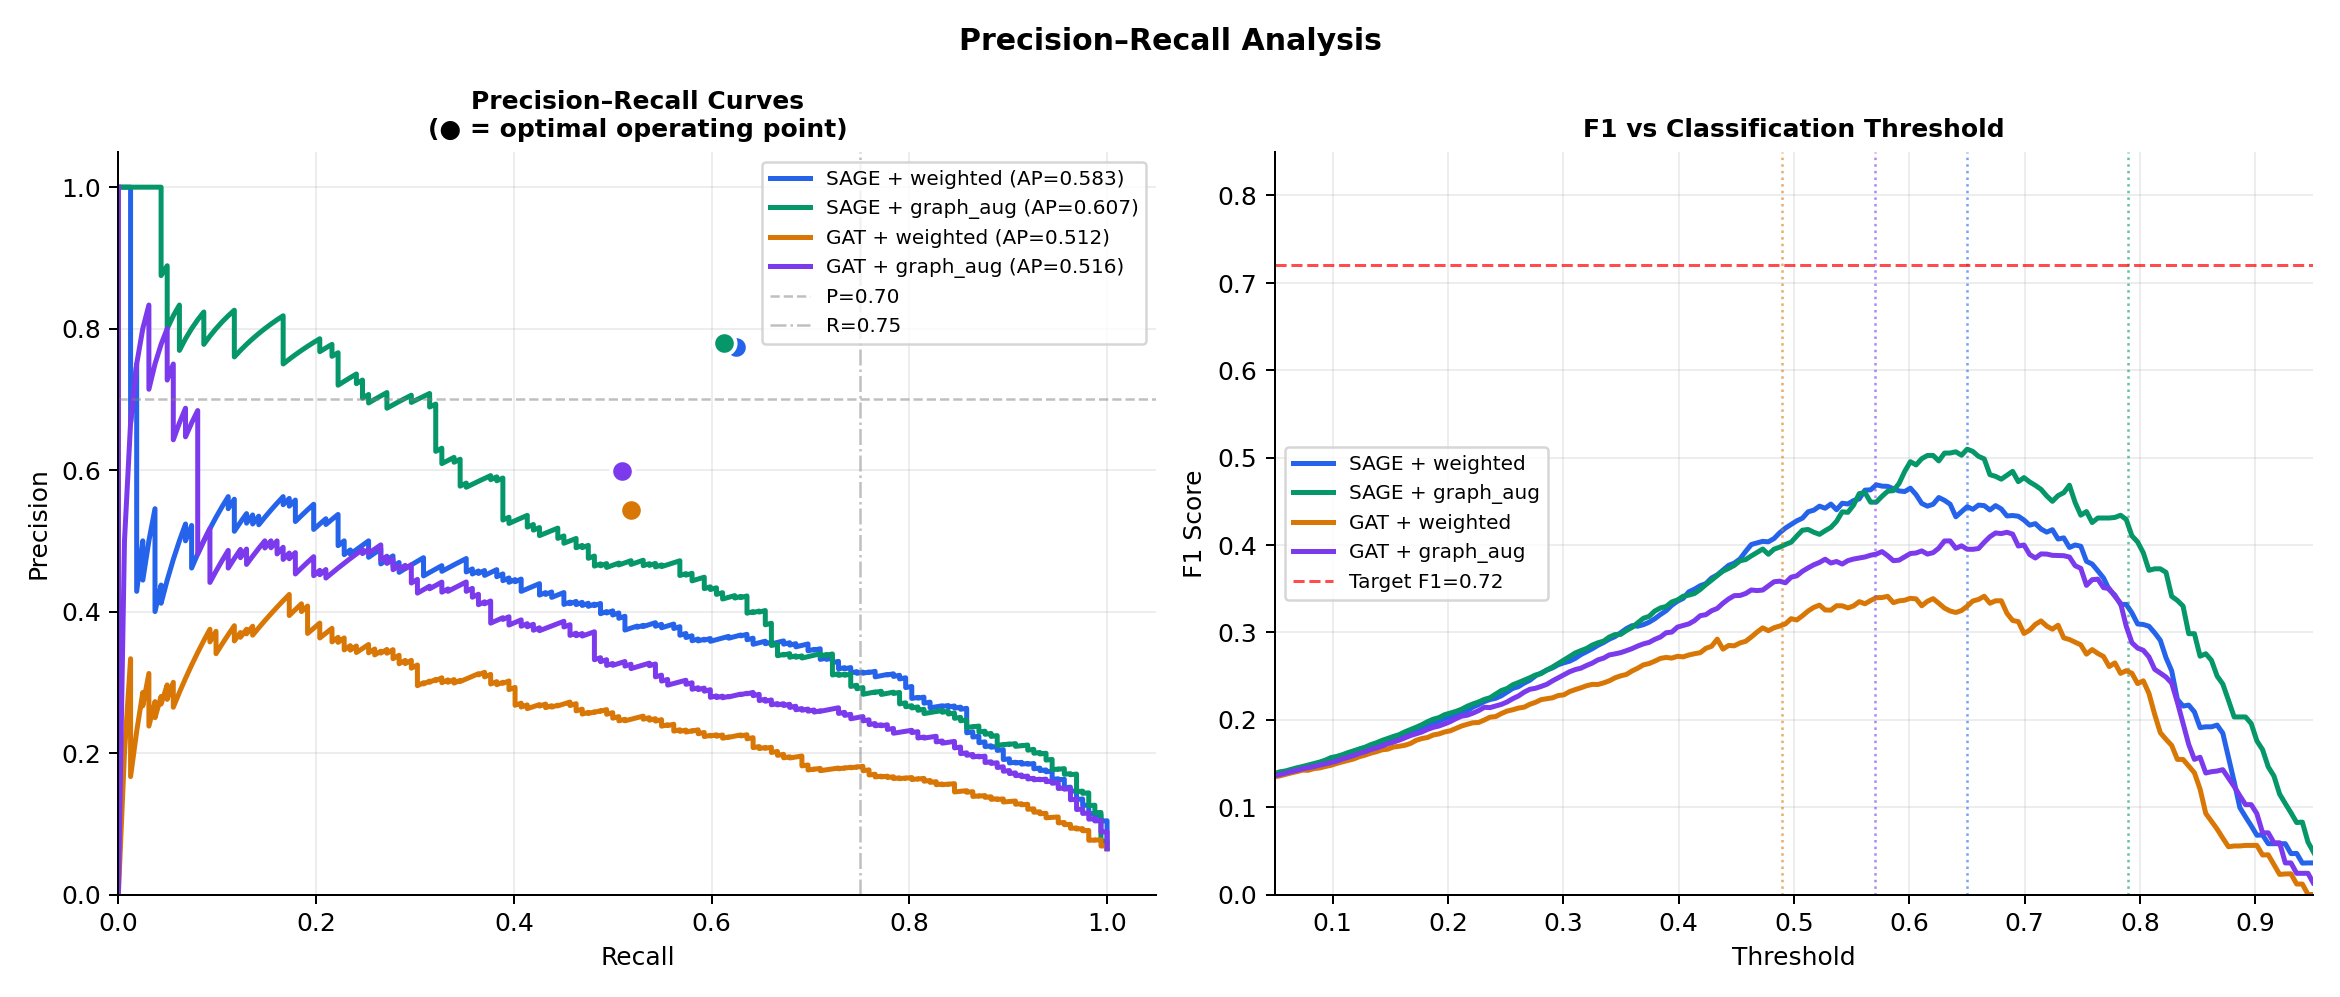
\includegraphics[width=\linewidth]{figures/fig6_pr_curves.png}\\[-0.2em]
  \footnotesize\textbf{(a)} Precision-recall curves.
\end{minipage}
\hfill
\begin{minipage}[b]{0.48\textwidth}
  \centering
  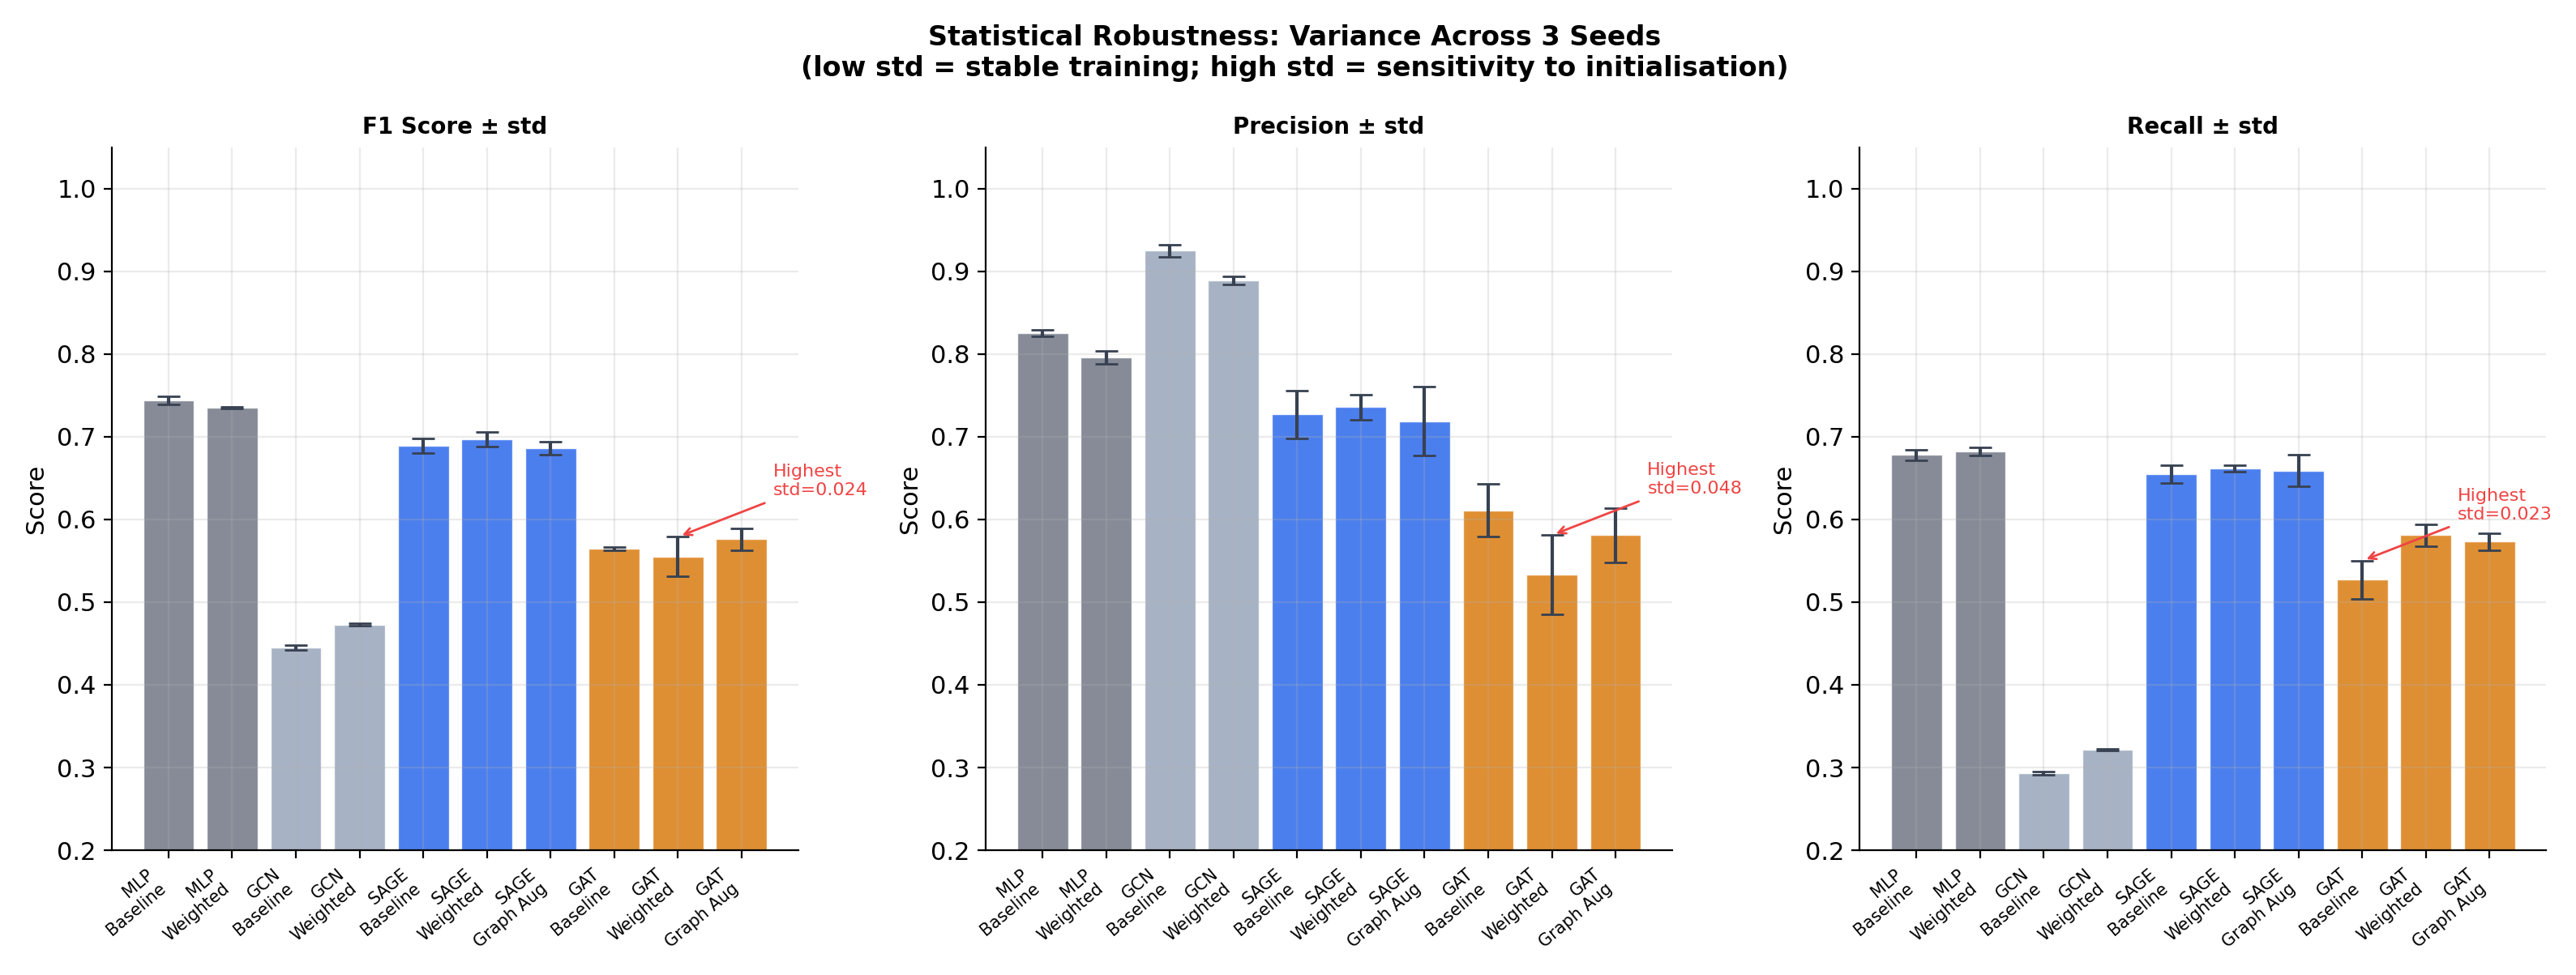
\includegraphics[width=\linewidth]{figures/fig15_variance_analysis.png}\\[-0.2em]
  \footnotesize\textbf{(b)} Seed variance across configurations.
\end{minipage}
\caption{Left: no threshold simultaneously achieves high precision
  and high recall. Right: MLP and SAGE are stable across seeds;
  GAT is the least stable family under imbalance.}
\label{fig:pr_cm}
\end{figure*}

%% ---------------------------------------------------------------
\section{Prior Work Comparison}
\label{sec:prior}

Table~\ref{tab:prior} compares our results to published Elliptic work.
All prior studies use GPU hardware and transductive evaluation. Our MLP
(F1\,=\,0.744) matches Alarab et al.\ (F1\,=\,0.740) under stricter
evaluation; our SAGE (F1\,=\,0.697) falls 5.3\,pp below Lo et al.\
(F1\,=\,0.750), largely attributable to the transductive-to-inductive
protocol gap.

\begin{table}[!t]
\centering
\caption{Prior Elliptic Work vs.\ This Study}
\label{tab:prior}
\scriptsize
\setlength{\tabcolsep}{3pt}
\begin{tabular}{llrll}
\toprule
\textbf{Work} & \textbf{Model} & \textbf{F1}
  & \textbf{HW} & \textbf{Protocol} \\
\midrule
Weber \cite{weber2019}    & GCN       & 0.700 & GPU & Transductive \\
Alarab \cite{alarab2020}  & GCN+feat  & 0.740 & GPU & Transductive \\
Lo \cite{lo2023}          & SAGE      & 0.750 & GPU & Transductive \\
Pareja \cite{pareja2020evolvegcn} & EvolveGCN & 0.770 & GPU
  & Temporal \\
\midrule
\textbf{Ours} & \textbf{MLP} & \textbf{0.744$\pm$.005}
  & CPU & Inductive \\
Ours & SAGE & 0.697$\pm$.009 & CPU & Inductive \\
Ours & RF (no graph) & \textbf{0.820} & CPU & Inductive \\
Ours (ablation) & EvolveGCN & 0.290 & CPU & Sampled \\
\bottomrule
\end{tabular}
\end{table}

%% ---------------------------------------------------------------
\section{Discussion and Conclusion}
\label{sec:conclusion}

\textbf{Practical implications.} Three findings bear on deployment.
First, periodic retraining is mandatory: a 39$\times$ fraud-rate
decline cannot be addressed by any static model or post-hoc
calibration. Sliding-window retraining is the minimum practical
requirement. Second, graph structure is a conditional asset:
beneficial during stable periods, harmful under rapid distributional
shift. Adaptive monitoring that switches between structural and
feature-only prediction could capture both benefits. Third, business
cost functions should drive deployment decisions. The highest-F1 model
(MLP, 0.744) is not the cheapest to deploy under asymmetric FN/FP
penalties (GAT + Graph Aug.\ costs less). F1 alone is an incomplete
guide to operational value.

The hybrid result adds a fourth point: GNN-derived representations
carry complementary signal even when the GNN fails as a standalone
classifier. The concat hybrid (F1\,=\,0.807) approaches the RF
ceiling (0.820), reframing the question from whether GNNs outperform
MLPs to how graph-learned features should be integrated into
production pipelines.

\textbf{Limitations.} RandomNodeLoader rather than NeighborLoader
(missing \texttt{torch-sparse} on M4 CPU) may underestimate GNN
performance by 5--10\,pp. Results come from one dataset; the
EvolveGCN result is a hardware lower bound. Three-seed validation
has limited statistical power.

\textbf{Conclusion.} Under inductive evaluation on the Elliptic
Bitcoin Dataset, a plain MLP (F1\,=\,0.744) outperforms all tested
GNNs. An RF baseline with no graph achieves F1\,=\,0.820. Temporal
distribution shift (fraud rate 11.6\,\% $\to$ 0.3\,\%) causes
near-complete recall failure for every model after step~42.
Graph-structure ablation shows shuffled edges outperform the real
transaction graph ($\Delta$F1\,=\,+0.116). Temperature scaling
confirms a structural root cause ($\Delta$F1\,=\,0). Yet a
concatenation hybrid recovers F1\,=\,0.807 by fusing GNN embeddings
with raw features, showing that graph-derived representations retain
value when properly integrated. These findings argue for hybrid
architectures, periodic retraining, and cost-aware model selection
in production fraud detection systems.

\bibliographystyle{IEEEtran}
\bibliography{references}

\end{document}
